%% 
%% Copyright 2007-2020 Elsevier Ltd
%% 
%% This file is part of the 'Elsarticle Bundle'.
%% ---------------------------------------------
%% 
%% It may be distributed under the conditions of the LaTeX Project Public
%% License, either version 1.2 of this license or (at your option) any
%% later version.  The latest version of this license is in
%%    http://www.latex-project.org/lppl.txt
%% and version 1.2 or later is part of all distributions of LaTeX
%% version 1999/12/01 or later.
%% 
%% The list of all files belonging to the 'Elsarticle Bundle' is
%% given in the file `manifest.txt'.
%% 
%% Template article for Elsevier's document class `elsarticle'
%% with harvard style bibliographic references

\documentclass[preprint,12pt]{elsarticle}

%% Use the option review to obtain double line spacing
%% \documentclass[preprint,review,12pt]{elsarticle}

%% Use the options 1p,twocolumn; 3p; 3p,twocolumn; 5p; or 5p,twocolumn
%% for a journal layout:
%% \documentclass[final,1p,times]{elsarticle}
%% \documentclass[final,1p,times,twocolumn]{elsarticle}
%% \documentclass[final,3p,times]{elsarticle}
%% \documentclass[final,3p,times,twocolumn]{elsarticle}
%% \documentclass[final,5p,times]{elsarticle}
%% \documentclass[final,5p,times,twocolumn]{elsarticle}

%% For including figures, graphicx.sty has been loaded in
%% elsarticle.cls. If you prefer to use the old commands
%% please give \usepackage{epsfig}

%% The amssymb package provides various useful mathematical symbols
\usepackage{amssymb}
%% The amsthm package provides extended theorem environments
%% \usepackage{amsthm}

%% The lineno packages adds line numbers. Start line numbering with
%% \begin{linenumbers}, end it with \end{linenumbers}. Or switch it on
%% for the whole article with \linenumbers.
%% \usepackage{lineno}
\usepackage{color}
\usepackage{xcolor}
\usepackage{subfigure}
\usepackage[hidelinks]{hyperref}
\usepackage[printonlyused]{acronym}
\usepackage{listings}
\usepackage{algorithm,algpseudocode}
%\usepackage{math}
\usepackage{tikz}
\usepackage{pgfplots}

\journal{Computer Physics Communications}

\lstset{
    showstringspaces=false,
    extendedchars=true,
    basicstyle=\footnotesize\ttfamily,
    commentstyle=\slshape,
    stringstyle=\ttfamily,
    breaklines=true,
    breakatwhitespace=true,
    columns=flexible,
    numbers=left,
    numberstyle=\tiny,
    basewidth=.5em,
    xleftmargin=.5cm,
    captionpos=b,
    frame=lines
}

%Predefined commands
\newcommand{\bq}{\begin{equation}}
\newcommand{\eq}{\end{equation}}
\newcommand{\bytes}{\mbox{bytes}}
\newcommand{\byte}{\mbox{byte}}
\newcommand{\second}{\mbox{s}}
\newcommand{\seconds}{\mbox{s}}
\newcommand{\flop}{\mbox{flop}}
\newcommand{\flops}{\mbox{flops}}
\newcommand{\NJFLOP}{\mbox{nJ/\flop}}
\newcommand{\instr}{\mbox{instr}}
\newcommand{\cycle}{\mbox{cy}}
\newcommand{\iter}{\mbox{it}}
\newcommand{\cycles}{\mbox{cy}}
\newcommand{\FCY}{\mbox{\flop/\cycle}}
\newcommand{\FIT}{\mbox{\flop/\iter}}
\newcommand{\BIT}{\mbox{\byte/\iter}}
\newcommand{\FR}{\mbox{\flops/\mbox{row}}}
\newcommand{\BR}{\mbox{\byte/\mbox{row}}}
\newcommand{\CYF}{\mbox{\cycles/\flop}}
\newcommand{\CS}{\mbox{\cycle/\second}}
\newcommand{\GCS}{\mbox{G\cycle/\second}}
\newcommand{\word}{\mbox{Word}}
\newcommand{\words}{\mbox{Words}}
\newcommand{\order}[1]{\mbox{${\cal O}\left(\mbox{#1}\right)$}}
\newcommand{\bit}{\mbox{bit}}
\newcommand{\bits}{\mbox{bits}}
\newcommand{\GBPS}{\mbox{G\bit/\second}}
\newcommand{\MBPS}{\mbox{M\bit/\second}}
\newcommand{\FS}{\mbox{\flop/\second}}
\newcommand{\BS}{\mbox{\byte/\second}}
\newcommand{\BC}{\mbox{\byte/\cycle}}
\newcommand{\GBS}{\mbox{G\byte/\second}}
\newcommand{\MBS}{\mbox{M\byte/\second}}
\newcommand{\GWS}{\mbox{G\word/\second}}
\newcommand{\GFS}{\mbox{G\flop/\second}}
\newcommand{\MFS}{\mbox{M\flop/\second}}
\newcommand{\lup}{\mbox{LUP}}
\newcommand{\lups}{\mbox{LUPs}}
\newcommand{\LUPCY}{\mbox{\lup/\cycle}}
\newcommand{\LUPS}{\mbox{\lup/\second}}
\newcommand{\MLUPS}{\mbox{M\lup/\second}}
\newcommand{\GLUPS}{\mbox{G\lup/\second}}
\newcommand{\GHZ}{\mbox{GHz}}
\newcommand{\ns}{\mbox{ns}}
\newcommand{\WF}{\mbox{\word/\flop}}
\newcommand{\BF}{\mbox{\byte/\flop}}
\newcommand{\FB}{\mbox{\flop/\byte}}
\newcommand{\BL}{\mbox{\byte/\lup}}
\newcommand{\GB}{\mbox{GB}}
\newcommand{\KB}{\mbox{kB}}
\newcommand{\MB}{\mbox{MB}}
\newcommand{\GiB}{\mbox{GiB}}
\newcommand{\MiB}{\mbox{MiB}}
\newcommand{\KiB}{\mbox{KiB}}
\newcommand{\W}{\mbox{W}}
\newcommand{\muarch}{\mbox{$\mu$-arch}}
\newcommand{\muop}{\mbox{$\mu$-op}}
\newcommand{\muops}{\mbox{$\mu$-ops}}
\newcommand{\eos}{\;.}
\newcommand{\cma}{\;,}
\newcommand{\rlm}{roof{}line model}
\newcommand{\rl}{roof{}line}
\newcommand{\Rlm}{Roof{}line model}
\newcommand{\Rl}{Roof{}line}
\newcommand{\olsep}{\|}
\newcommand{\nolsep}{|}
\newcommand{\ecmspace}{\,}
\newcommand{\TOL}{$T_{\mathrm{c}\_\mathrm{OL}}$}
\newcommand{\NNZR}{$N_\mathrm{nzr}$}
\newcommand{\NR}{$N_\mathrm{r}$}
\newcommand{\NNZ}{$N_\mathrm{nz}$}
\newcommand{\ecm}[6]{\mbox{$\left\{{#1}\ecmspace\olsep\ecmspace {#2}\ecmspace\nolsep\ecmspace {#3}\ecmspace\nolsep\ecmspace {#4}\ecmspace\nolsep\ecmspace {#5}\right\}\ecmspace{#6}$}}
\newcommand{\epsep}{\rceil}
\newcommand{\ecmp}[4]{\mbox{$\left\{{#1}\ecmspace\epsep\ecmspace {#2}\ecmspace\epsep\ecmspace {#3}\right\}\ecmspace{#4}$}}
\newcommand{\ecme}[4]{\mbox{$\left({#1}\ecmspace\epsep\ecmspace {#2}\ecmspace\epsep\ecmspace {#3}\right)\ecmspace{#4}$}}
\newcommand{\sellcs}{SELL-\texorpdfstring{$C$-$\sigma$}{C-sigma}}
\newcommand{\likwid}{\texttt{LIKWID}}
\newcommand{\likwidperfctr}{\texttt{likwid-perfctr}}
\newcommand{\likwidpin}{\texttt{likwid-pin}}
\newcommand{\likwidbench}{\texttt{likwid-bench}}
\newcommand{\lmbench}{\texttt{lmbench}}

% Acronyms
\newacro{AoS}{array of structures}
\newacro{AoSoA}{array of structures of arrays}
\newacro{CPI}{cycles per instruction}
\newacro{DEM}{discrete element method}
\newacro{EAM}{embedded atom method}
\newacro{FCC}{face-centered cubic}
\newacro{FN}{full neighbor-lists}
\newacro{HN}{half neighbor-lists}
\newacro{ILP}{instruction-level parallelism}
\newacro{IR}{intermediate representation}
\newacro{AST}{abstract syntax tree}
\newacro{ISA}{instruction set architecture}
\newacro{LJ}{Lennard-Jones}
\newacro{MD}{Molecular dynamics}
\newacro{MPI}{message passing interface}
\newacro{SIMD}{single instruction, multiple data}
\newacro{SoA}{structure of arrays}
\newacro{PBC}{periodic boundary conditions}
\newacro{HPM}{hardware performance monitoring}

\begin{document}

\begin{frontmatter}

%% Title, authors and addresses

%% use the tnoteref command within \title for footnotes;
%% use the tnotetext command for theassociated footnote;
%% use the fnref command within \author or \address for footnotes;
%% use the fntext command for theassociated footnote;
%% use the corref command within \author for corresponding author footnotes;
%% use the cortext command for theassociated footnote;
%% use the ead command for the email address,
%% and the form \ead[url] for the home page:
%% \title{Title\tnoteref{label1}}
%% \tnotetext[label1]{}
%% \author{Name\corref{cor1}\fnref{label2}}
%% \ead{email address}
%% \ead[url]{home page}
%% \fntext[label2]{}
%% \cortext[cor1]{}
%% \affiliation{organization={},
%%             addressline={},
%%             city={},
%%             postcode={},
%%             state={},
%%             country={}}
%% \fntext[label3]{}

\title{P4IRS: An Intermediate Representation and Compiler for Parallel and Performance-Portable Particle Simulations}

%% use optional labels to link authors explicitly to addresses:
%% \author[label1,label2]{}
%% \affiliation[label1]{organization={},
%%             addressline={},
%%             city={},
%%             postcode={},
%%             state={},
%%             country={}}
%%
%% \affiliation[label2]{organization={},
%%             addressline={},
%%             city={},
%%             postcode={},
%%             state={},
%%             country={}}

\author[nhratfau]{Rafael Ravedutti Lucio Machado\corref{cor1}}
\cortext[cor1]{Corresponding author. E-mail address: rafael.r.ravedutti@fau.de, Tel.: +49 9131 85-27927, Fax: +49 9131 85-28928}
\author[nhratfau]{Jan Eitzinger}
\author[nhratfau]{Harald Köstler}

\affiliation[nhratfau]{
	organization={Erlangen National High Performance Computing Center}, %(NHR@FAU)},
	addressline={Martensstraße 1},
	city={Erlangen},
	postcode={91058},
	state={Bayern},
	country={Germany}}

\begin{abstract}
Various physics simulations today rely on simulating particle interactions, where particles can represent point masses (as in Molecular Dynamics), rigid bodies (as in Discrete Element Method) or even massive bodies such as planets.
Evaluating and calculating the required particle interactions in a simulation is computationally expensive, hence suitable algorithms and proper optimizations to exploit available parallelism in the target hardware are important to reach good performance.
However, it is difficult to maintain flexible implementations while keeping state-of-the-art performance, as most packages are developed individually and have their own hard-coded, fine-tuned implementations.
To combine flexibility and optimal performance, we introduce P4IRS, an intermediate representation and compiler for particle simulations which is aimed at delivering good performance.
We describe P4IRS, display usage examples and features, discussing the benefits we can obtain with code generation.
Finally, we evaluate the performance and scalability from the code generated by P4IRS on modern processors, accelerators and supercomputers in both MD and DEM fields.
\end{abstract}

%%Graphical abstract
\begin{graphicalabstract}
%\includegraphics{grabs}
\end{graphicalabstract}

%%Research highlights
\begin{highlights}
\item A DSL and code generator for performance-portable particle simulations is introduced
\item Different algorithms such as Linked Cells and Verlet Lists can be generated
\item Generated codes can solve Molecular Dynamics and Discrete Element Method simulations
\item Base and scaling performances are shown for CPUs and GPUs in both Fritz and JUWELS-Booster clusters
\item Optimization aspects and strategies of Molecular Dynamics and Discrete Element Method simulations are discussed
\end{highlights}

\begin{keyword}
%% keywords here, in the form: keyword \sep keyword

%% PACS codes here, in the form: \PACS code \sep code

%% MSC codes here, in the form: \MSC code \sep code
%% or \MSC[2008] code \sep code (2000 is the default)
code generation \sep particle simulations \sep molecular dynamics \sep discrete element method \sep HPC
\end{keyword}

\end{frontmatter}

%% \linenumbers

%% main text
\section{Introduction}
\label{sec:introduction}

The computation of particle-pair interactions is widely used in physics simulations, especially in the fields of Molecular Dynamics and Discrete Element Method.
To efficiently compute the inter-particle contributions, different strategies can be used to increase efficiency and make use of the parallelism offered by the target hardware.
Most simulation packages, however, have their own hard-coded implementations, which are strictly tightened to their data structures and programming artifacts.
Also, several kernel implementations for the same potential or force field are present in a single package to account for different hardwares and optimizations strategies, leading to higher maintainability costs and higher portability effort.

To tackle these limitations, we developed P4IRS --- Parallel and Performance-Portable Particles Intermediate Representation and Simulator, an intermediate representation and compiler tool where particle interactions can be simply expressed as Python methods, and efficient and parallel code for the interaction description can be generated for multi-CPU and multi-GPU targets.
P4IRS provide its own intermediate representation, which allows it to perform compiler analysis and transformations, to then generate code for the proper backend such as C++ and CUDA with OpenMP/MPI.

P4IRS can generate several kernel flavours of the same potential such as Linked Cells \cite{linkedcells} and Verlet Lists \cite{verletlists}, where data layouts for properties and specific arrays (such as the neighbor-lists) can be switched to the case with best performance.
A runtime interface in C++ is also available and can be used to integrate P4IRS with other simulation tools, which is particularly important for integrating P4IRS simulations with our multi-physics framework waLBerLa \cite{walberla1,walberla2}.
%as an example we show how P4IRS can use the load-balancing communication algorithm from waLBerLa to compute simulations with a more heterogeneous distribution of particles.

Most of P4IRS internal routines such as building Linked Cells and Verlet Lists are implemented in Python by constructing the intermediate representation for them with the assistance of operator overloading (see \autoref{sec:backend}).
In this way, we leverage P4IRS analysis and transformations to achieve performance-portability for these routines as well, without requiring multiple tailored implementations.

The goals of this paper are summarized as follows:
\begin{itemize}
	\item We present our code generator tool P4IRS, describing how it works and how it can be used to generate efficient particle simulation codes.
	\item We discuss the advantages of using P4IRS to achieve performance-portability, also comparing it with other previous approaches such as tinyMD \cite{tinymd} and MESA-PD \cite{mesapd1,mesapd2}.
	\item We describe P4IRS interfaces to allow its generated code to be integrated with other simulation tools, specifically in the context of domain-partitioning and communication.
	\item We provide performance results for Intel Ice Lake and AMD Milan CPUs, as well as for NVIDIA A40 and A100 accelerators to demonstrate the state-of-the-art performance of the applications generated by P4IRS in comparison to MD-Bench and MESA-PD.
	\item We display weak-scaling results in the Fritz and JUWELS Booster clusters to demonstrate the weak-scaling capabilities of P4IRS in MD and DEM simulations on modern supercomputers.
\end{itemize}

This paper is structured as follows: In \autoref{sec:related_work} we list related work for MD and DEM simulation packages, code generation tools for particle simulations and performance evaluation of such simulations. In \autoref{sec:background} we explain the basic theory for particle simulations focusing on MD and DEM methods, also covering optimization strategies and choices. In \autoref{sec:pairs} we present P4IRS with its current features and application design. In \autoref{sec:evaluation} we evaluate the performance and scalability from P4IRS applications using \ac{MD} and \ac{DEM} experiments. Finally, \autoref{sec:conclusion} presents our conclusion and outlook for P4IRS, also covering our future work.

\section{Related Work}
\label{sec:related_work}

\subsection{Simulation Packages}
\label{sec:packages}

Diverse simulation fields can be described by updating particle trajectories based on their interactions with other particles.
In this paper, we mainly focus on \ac{MD} and \ac{DEM}, where particles represent either point masses (i.e. atoms) and rigid bodies with specific shapes (i.e. spheres, half-spaces, ellipses), respectively.
Most packages available use similar techniques to compute trajectories, but each of them have their own specific algorithms, parallelism strategies and hand-tuned implementations for specific hardware.
With P4IRS, we focus on using a single description of the problem, and then leverage its implemented routines and code transformations to produce the backend implementation for the specific target, which currently can be C++ with OpenMP and CUDA, also supporting MPI for distributed-memory parallel clusters.

In MD, there exist many packages with distinct strategies and simulation fields.
LAMMPS \cite{lammps1,lammps2} is a molecular package for the material-modeling field which uses the standard Verlet Lists algorithm to optimize the non-bonded short-range force calculations.
It offers many inter-atomic potentials, each one with different kernel implementations for a specific target (like CPU, GPU or Kokkos \cite{kokkos}).
GROMACS \cite{gromacs1,gromacs2} is another package for MD with focus on bio-sciences simulation which uses its own Cluster Pair algorithm to optimize the short-range forces computation.
It does not support as many potentials as LAMMPS, but its algorithm tends to be significantly faster than the Verlet Lists since it employs SIMD parallelism more efficiently.
Furthermore, the optimal GROMACS kernel implementations rely on SIMD intrinsics to attain higher performance, which makes them harder to be maintained and ported to other architectures.
Also, the GPU algorithm in GROMACS differs from the CPU, since it relies on a strategy named ``super-clustering'' to reduce the amount of redundant computations caused by adjusting the cluster sizes to fit the SIMD width in the GPU.
Other MD packages such as HOOMD-blue \cite{hoomdblue}, NAMD \cite{namd}, AMBER \cite{amber1,amber2} and CHARMM \cite{charmm} also contain dedicated and hand-tuned implementations in general purpose languages for each supported backend.
Each version is tested, maintained, debugged and optimized independently.

Packages that support DEM simulations are in general more flexible (since simulation with more particle properties such as rotations and shapes are needed), however they usually do not have the same optimization techniques as the MD simulation packages.
The reason is most likely that it is not so feasible to support flexibility with sophisticated optimization algorithms as the complexity of the code grows considerably.
Examples of such packages are the LIGGGHTS DEM \cite{liggghts} (based on LAMMPS), MercuryDPM \cite{mercurydpm} and YADE \cite{yade}.
To mitigate such limitations, a few code generation approaches were developed for both MD and DEM.

\subsection{Code Generation Frameworks}
\label{sec:codegen}

% TODO: OpenMM, MDL, ppmd, OpenFPM, PPME
% TODO: MESA-PD, tinyMD

Solutions based on code generation are also available for specific fields of particle simulations, and these aim at providing a higher level of flexibility and extensibility while strive for efficient performance in modern accelerators.

OpenMM \cite{openmm} is a \ac{MD} package that makes use of Python as a front-end for simulation protocols and file I/O, it contains a C++ API for forces and integrators as well as optimized kernel implementations for CUDA, C++ and OpenCL.
Integrators and forces can be implemented by using mathematical descriptions in OpenMM, but its use cases are restricted to \ac{MD} simulations and several features required for a DEM simulation or other types of particles simulation (such as contact history and different shapes) are not available.

MESA-PD \cite{mesapd3} is a general particle dynamics framework that is built-in the waLBerla framework for the simulation of particles and fluids.
Its design principle of separation of code and data allows to introduce arbitrary interaction models with ease, which makes it also useful for \ac{MD}.
By using its code generation approach using Jinja templates it can be adapted very effectively to any simulation scenario.
As successor of the ``physics engine'' (pe) rigid particle dynamics framework it inherits its scalability and advanced load balancing functionalities.
One of the limitations of MESA-PD is that it does not support GPU code generation, and since its code generation approach is based on Jinja templates, the effort for implementing new functionalities may not be lower compared to other simulation packages without code generation techniques (for instance, most of its force kernels are not generated but rather implemented in C++).

In previous work we developed tinyMD, a proxy-app (also based on miniMD) created to evaluate the portability of MD and DEM applications with the AnyDSL \cite{anydsl1,anydsl2} framework.
TinyMD uses higher-order functions to abstract device iteration loops, data layouts and communication strategies, providing a domain-specific library to implement pair-wise interaction kernels that execute efficiently on multi-CPU and multi-GPU targets.
One of tinyMD's limitation is that its flexibility and optimization settings are restricted to what can be achieve through higher-order functions and the AnyDSL compilation framework (the generated LLVM IR restricts the backend compilation to the Clang compiler), overcoming such limitation is one of the reasons we develop P4IRS.


\subsection{Performance Evaluation}
\label{sec:perfeval}

Many performance-oriented researches exist for MD systems, most of them using MD packages as a black-box and adjusting different simulation parameters to analyse their implications in the overall performance.
In some cases, however, in-depth performance studies were made to gain a broader understanding on efficient ways to achieve SIMD vectorization with SSE/AVX instructions \cite{mdsimd}.
Most in-depth studies are performed using mini-apps or proxy-apps, one example is miniMD, a proxy-app that provides a simple copper face-cubic-centered lattice simulation where atom forces are computed with kernels extracted from LAMMPS for either the \ac{LJ} or \ac{EAM} potentials.

The Exascale Computing Project (ECP) Co-design Center for Particle Applications (CoPA) \cite{ecpcopa} focus on co-designing particle applications to prepare them for exascale computing.
They provide several proxy-apps for particle simulations such as CabanaMD and ExaMiniMD, which are designed in a modular fashion to account for different optimization strategies and particle data layouts, and also are built on top of Kokkos to be able to execute on many-core CPU and GPU targets.

Our performance-focused prototyping harness MD-Bench \cite{mdbench1,mdbench2} is a toolbox developed for performance-engineering \ac{MD} non-bonded short-range force calculation algorithms, with focus on in-core execution on CPUs and GPUs.
It currently supports the Verlet Lists and Cluster Pair algorithms from LAMMPS and GROMACS, respectively.
One of our goals is to use the knowledge obtained with MD-Bench and integrate it into P4IRS to achieve state-of-the-art performance and flexibility altogether in particle simulations.

Based on our searches, there are not many in-depth performance studies focusing on SIMD and in-core execution for kernels used in DEM simulations, and most existing studies focus on evaluating their distributed-memory parallelism in weak-scaling settings.
With P4IRS, we intend to bridge the gap between performance strategies across different simulation domains, and use the most efficient algorithm whenever it is possible without requiring significant efforts such as re-implementing kernels and re-designing applications with tailored data structures for improving performance.

To evaluate performance in a single CPU core or GPU in this paper, we use MD-Bench and miniMD as the baseline performance, as they are well-known implementations that reach state-of-the-art performance for MD simulations.
For DEM cases, we use MESA-PD as the comparison target, since our focus is to show that we can achieve performance-portability with the flexibility that MESA-PD provides. 

\section{Background and Theory}
\label{sec:background}

Particle simulations consist of solving N-body problems and have a wide range of applications as many fields can be represented as a system of interacting particles.
In this sense, particles can be either atoms, rigid bodies or even planets, stars and galaxies.
Interaction contributions can come either from inter-atomic van-der-Walls forces based on the \ac{LJ} potential, or even from gravitational forces generated by super-massive particles.
In order to simulate such systems, however, we need well-defined and closed system of particles with known boundary conditions.
In the scope of this paper, particle contributions are computed for particles that lie within a range or ``cutoff radius''. 
Strategies to compute approximations from particles beyond this range (also known as long-range contributions) also exist, but are not disclosed.
To provide distinct examples of simulations and demonstrate a certain level of flexibility from P4IRS, we focus on MD and DEM simulations in this work.

\subsection{Molecular Dynamics}
\label{sec:md}

\ac{MD} simulations are widely used today to study the behavior of microscopic structures.
These simulations reproduce the interactions among atoms in these structures on a macroscopic scale while allowing us to observe the evolution in the system of particles in a time-scale that is simpler to analyze.

Different areas such as material science to study the evolution of the system for specific materials, chemistry to analyze the evolution of chemical processes, or biology to reproduce the behavior of certain proteins and bio-molecules resort to simulations of \ac{MD} systems.

A \ac{MD} system to be simulated constitutes of a number of atoms, the initial state (such as the atoms' position or velocities), and the boundary conditions of the system.
Here, we use \ac{PBC} in all directions, hence when one atom crosses the domain, it reappears on the opposite side with the same velocity.
%These simulations are defined by establishing the number of atoms in a system, the initial state of the system (such as the atoms' positions or velocities), and the boundary conditions for the system.
Fundamentally, atom trajectories in classical \ac{MD} systems are computed by integrating Newton-Euler equations for every atom $i$:
\begin{equation}
    \hat F_i = m_i \dot{\hat v}_i \label{eq:newton_force}
\end{equation}
\begin{equation}
    \hat v_i = \dot{\hat x}_i \label{eq:newton_velocity}
\end{equation}
Where $m_i$, $\hat v_i$ and $\hat x_i$ are the mass, the velocity vector and the position vector of the atom $i$, respectively.
The force $F_i$ then must be calculated to integrate the positions of the atoms, and these are described by the negative gradient of the potential of interest.
The mutual force between atom $i$ and $j$ as governed by the \ac{LJ} potential
is given as:
\begin{equation}
    \hat{F}_{LJ}(\hat{x_i}, \hat{x_j}) = -\frac{24\varepsilon}{x_{ij}} \left( \frac{\sigma}{x_{ij}} \right)^{6} \left[ 2\left(\frac{\sigma}{x_{ij}}\right)^{6} - 1\right] \hat{x}_{ij}~,
    %V_{LJ} = 4\varepsilon \left[ \left(\frac{\sigma}{r}\right)^{12} - \left(\frac{\sigma}{r}\right)^6 \right]
    \label{eq:lennard_jones}
\end{equation}
Where $\hat{x}_{ij}$ is the distance vector between atoms $i$ and $j$, $x_{ij}$ is the distance between atoms $i$ and $j$, $\varepsilon$ is the width of the potential well, and $\sigma$ specifies at which distance the potential is~$0$.

\subsection{Discrete Element Method}
\label{sec:dem}

Besides computing trajectories for zero-dimensional point masses as done in MD, we can model particles as objects with specific shapes and spatial extension using the Discrete Element Method (DEM).
This requires support of more degrees of freedom for particles, since spatial properties (such as rotation) need to be taken into consideration.
In this work, we consider particles with homogeneous density, and then use the center of mass for each particle as its position, which coincides with its geometrical center due to its density properties.
Equations of motions are extended with the following terms for the torque and angular velocity:

\begin{equation}
    \hat{\tau}{_i} = I \dot{\hat \omega}_i + {\hat \omega}_i \times I {\hat \omega}_i \label{eq:newton_torque}
\end{equation}
\begin{equation}
    \hat{\omega}{_i} = \dot{\varphi}_i \label{eq:newton_angular_velocity}
\end{equation}

With the torque vector $\hat{\tau}{_i}$, angular velocity vector $\hat{\omega}{_i}$, rotation $\varphi$ (typically stored as a quaternion, rotation matrix or rotation vector) and moment of inertia about the center of mass $I = I(\varphi_i)$.
A collision detection step is required to check when two particles overlap, and parameters about the collision such as the contact point and penetration depth are computed and used in the force calculation.
Note that the reason a penetration occurs during a collision is that the collision is not detected right when it starts because the simulation is discretized by the time-step size.
For simplification purposes, we only calculate collision detections analytically in this work since there are no particles with complex shapes involved.

In this work, we use the penalty-based Linear Spring-Dashpot model to calculate forces among particles for the DEM cases.
The collision force is split into two components, one representing the force in the normal direction and one representing the force in the tangential direction.

The relative contact velocity $\hat{u}_{ij}$ is of importance for most contact models.
Considering $\hat{c}_{ij}$ the contact point and $\hat{n}_{ij}$ the normal direction vector between the particles $i$ and $j$, the relative contact velocity and its normal and tangential components $\hat{u}_{ij}^{n}$ and $\hat{u}_{ij}^{t}$ can be expressed as:


\begin{equation}
    \hat{u}_{ij} = \hat{v}_{i} - \hat{v}_{j} + \hat{\omega}_{i} \times (\hat{c}_{ij} - \hat{x}_{i}) - \hat{\omega}_{j} \times (\hat{c}_{ij} - \hat{x}_{j})
    \label{eq:relative_contact_velocity}
\end{equation}

\begin{equation}
    \hat{u}_{ij}^{n} = \hat{u}_{ij} \cdot \hat{n}_{ij} * \hat{n}_{ij}
    \label{eq:relative_contact_velocity_n}
\end{equation}

\begin{equation}
    \hat{u}_{ij}^{t} = \hat{u}_{ij} - \hat{u}_{ij}^{n}
    \label{eq:relative_contact_velocity_t}
\end{equation}

Then, the force components in the normal direction $\hat{F}_{SD}^{n}$ and in the tangential direction $\hat{F}_{SD}^{t}$ can be defined as:

\begin{equation}
    \hat{F}_{SD}^{n}(\hat{x_i}, \hat{x_j}) = k^{n}\delta_{ij}\hat{n}_{ij} - \xi^{n}\hat{u}_{ij}^{n}
    \label{eq:linear_spring_dashpot_normal}
\end{equation}

\begin{equation}
    \hat{F}_{SD}^{t}(\hat{x_i}, \hat{x_j}) = -\min \left\{ k^{t}\left| \delta^{t}_{ij} \right|,\mu\left|\hat{F}_{SD}^{n}(\hat{x_i}, \hat{x_j}) \right| \right\} \hat{\delta}^{t}_{ij}
    \label{eq:linear_spring_dashpot_tangential}
\end{equation}

\begin{equation}
    \hat{\delta}^{t}_{ij} \gets \hat{\delta}^{t}_{ij} + \hat{u}_{ij}^{t}dt
    \label{eq:update_rule}
\end{equation}

Where $k^{n}$ is the normal spring stiffness, $k^{t}$ the tangential spring stiffness, $\xi^{n}$ the normal velocity damping, $\mu$ the friction, $\delta_{ij}$ the penetration depth and $dt$ the time-step size.
The update rule in \autoref{eq:update_rule} and modifications in \autoref{eq:linear_spring_dashpot_tangential} were properly included to fix frictional contact accordingly \cite{dem1,dem2}.
The tangential spring displacement $\hat{\delta}^{t}_{ij}$ is initialized as a zero vector in the first contact between the particles $i$ and $j$, and the update rule is carried out every time-step the contact persists.
From the algorithmic point of view, this means that a contact history data structure is required to keep track of the last computed value for every pair of particles that are in contact.

\subsection{Optimization Strategies}
\label{sec:opts}

\begin{figure*}[htb]
    \centering
    \subfigure[Linked Cells]{\label{fig:linked_cells}\includegraphics[width=0.40\textwidth]{linked_cells.pdf}}
    \subfigure[Verlet Lists]{\label{fig:verlet_lists}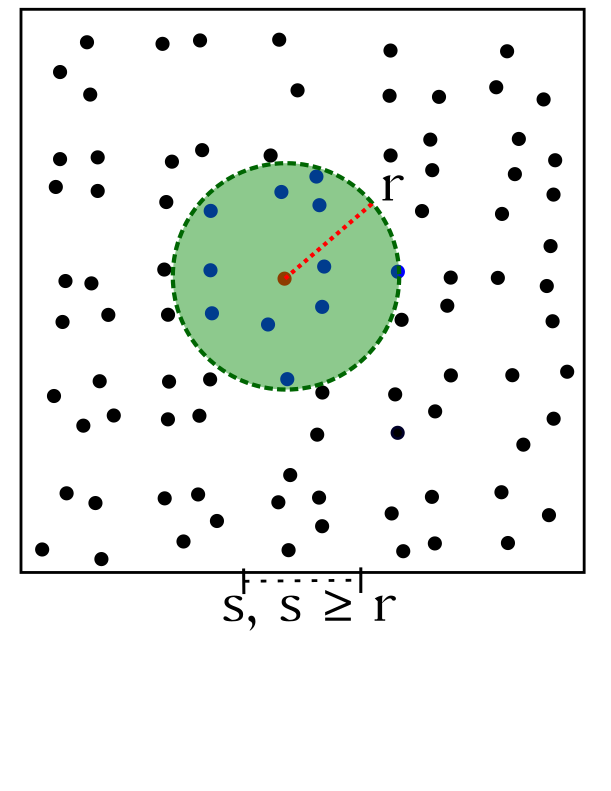
\includegraphics[width=0.40\textwidth]{verlet_lists.pdf}}
    \caption{Comparison between (a) Linked Cells and (b) Verlet Lists algorithms, in each case, the blue particles are used as the candidates to compute the forces with the red particle. In the Linked Cells, all particles in the neighbor cells are considered (considering the size of the cell is higher or equal than the cutoff radius). In the Verlet Lists, a list of particles is created by evaluating which particle distances are smaller than the cutoff radius plus a "skin" value, which represents a sphere in the 3D case.}
\end{figure*}

To calculate the resulting force for a particle in a specific time-step, it is necessary to compute all partial force contributions from each of the other particles present in the system.
In a naive strategy, this results in a quadratic complexity and severely affects the application performance, which limits the system size and the time-scale of the simulation.

When force contributions become negligible at long-distance interactions or when a contact between particles is needed, different algorithm strategies can be employed to perform computations only for particles within a specific cut-off region.
There are two main data structures which are commonly used for efficiently computing particle interactions in state-of-the-art simulation packages: the Linked Cells and the Verlet Lists.

Linked Cells strategy (see Figure~\ref{fig:linked_cells}) sorts particles spatially according to their position in cells (also called bins), where cells have a fixed size, and mapping particles into cells can be done directly by computing in which cell a particle is contained within.
After, forces can be computed for each particle by traversing its current and neighbor cells, and only adding contributions for particles within these cells.

The Linked Cells results in computing only forces for particles within a region that is discretized by their current and neighbor cells/bins, which can still results in a significant amount of redundant computations.
In order to avoid even more redundant computations, the Verlet Lists strategy can be used jointly with Linked Cells.
The Verlet Lists (see Figure~\ref{fig:verlet_lists}) constructs a list of neighbor particles for every particle, and this list can be created by using the Linked Cells structure, evaluating the distances among particles within close bins and then using the distance to determine whether such particles should be added into the list.
In the Verlet Lists case, the region for searching for neighbor particles is defined by a sphere, where the center of the sphere is the position of the particle and the radius is the cutoff radius plus a "skin".
The "skin" is used to avoid building the neighbor-lists at every time-step, it extends the neighbor-search and avoid missing computations from particles that end up entering the cut-off region in subsequent time-steps in which the neighbor-lists are not reconstructed.

Despite avoiding computations from long-distance particles, another common optimization is to take advantage of Newton's Third Law and compute forces in only one direction.
This means that only half of particle-pairs are traversed when computing the forces, and partial forces are decreased for the neighbor particles during their computation.
Ideally, this should lead to a factor of two speedup, but this strategy has a few drawbacks: (a) parallelism is harmed since decreasing force of neighbor particles requires atomic operations to avoid race conditions and (b) when the code is vectorized with SIMD intrinsics (such as AVX2 and AVX512), gather and scatter instructions are needed to build up the SIMD registers with forces of the neighbor particles, which results in scattered memory accesses and extra instructions.
At the end, this strategy is likely to be beneficial for more arithmetic-intensive kernels, and the trade-off between parallelism and less arithmetic operations must be assessed to know when it is advantageous.

\section{P4IRS}
\label{sec:pairs}

% Show examples (LJ, EAM)
% Linked Cells / Verlet Lists
% Can generate CPU/GPU code
% Vectors, quaternions and matrices
% Properties, feature properties and contact properties
% Contact history
% Shape partitioning

\begin{figure*}[htb]
  \centering
  \includegraphics[width=0.9\textwidth]{pairs_overview.png}
  \caption{Overview of P4IRS architecture.}
  \label{fig:features}
\end{figure*}

P4IRS\footnote{\url{https://i10git.cs.fau.de/software/pairs}} is an open-source, stand-alone compiler and domain-specific language for particle simulations which aims at generating optimized code for different target hardwares.
It is released as a Python package and allows users to define kernels, integrators and other particle routines in a high-level and straightforward fashion without the need to implement any backend code.

\autoref{fig:features} displays an overview of P4IRS.
In the left side, the front-end library from P4IRS is displayed with the available features, all these are defined through a Python interface by the user for modeling the simulation and determining the optimization schedule.
In the middle, the backend with the internal methods (deep-embedded in Python) with the compiler transformations and analyses are shown, these make use of the front-end representation to produce the final backend code.
In the right side, the final generated code is integrated and compiled together with the runtime modules and functionalities to achieve parallelism and accesses to external features.
The next subsections explore the different P4IRS features in more detail.

\subsection{Frontend and Features}
\label{sec:frontend}

\autoref{lst:pairslj} shows a simple description in P4IRS to compute forces with the \ac{LJ} potential.
Functions can be provided through a method (line 1), and the parameters in the method refer to different particles in the system.
In this way, many-body potentials can also be described using methods with more than two parameters.
Some keywords are also provided by P4IRS for writing the kernels, in line 2 the \emph{squared\_distance} method is used for obtaining the squared distance for the atoms \emph{i} and \emph{j}, and in line 4 the \emph{delta} method is used for obtaining the delta vector.
Also, in lines 3 and 4 it is possible to see accesses to feature properties called \emph{sigma6} and \emph{epsilon}, which are defined during the simulation setup as properties which depend on the atom types feature.
In line 4, the \emph{apply} method is used for applying the computed term into the \emph{force} property of the particles, the method allows the identification of particle properties reductions and is also used when generating the kernel variant using the half neighbor-lists.

\begin{lstlisting}[language=Python,
		   label={lst:pairslj},
		   caption={Lennard-Jones force description in P4IRS.}]
def lennard_jones(i, j):
    sr2 = 1.0 / squared_distance(i, j)
    sr6 = sr2 * sr2 * sr2 * sigma6[i, j]
    apply(force, delta(i, j) * (48.0 * sr6 * (sr6 - 0.5) * sr2 * epsilon[i, j]))
\end{lstlisting}

Functions that update every particle separately can also be described with a single parameter.
\autoref{lst:euler} displays how to implement a simple Euler integrator for \ac{MD} (see line 1).
In lines 2-3, there are also property accesses for the particles' linear velocities, forces, masses and positions.
Note that vector operations are intrinsically supported in P4IRS, which is also the case for matrices and quaternions data structures.
P4IRS methods also allow the specification of parameters such as the \emph{dt} specified in line 3, these must be given when setting up the simulation.

\begin{lstlisting}[language=Python,
		   label={lst:euler},
		   caption={Euler integrator description in P4IRS.}]
def euler(i):
    linear_velocity[i] += dt * force[i] / mass[i]
    position[i] += dt * linear_velocity[i]
\end{lstlisting}

\autoref{lst:pairs_md_setup} shows the simulation setup for the \ac{MD} case. In the first part (lines 6-10), a \emph{simulation} instance is created, and its identifier, the list of particle shapes used, the number of time-steps and the floating-point precision are specified.
Further, the properties needed for each particle in the simulation are specified (lines 13-16), together with their data types and (if needed) initial values.
Some properties are also defined as volatile (in this case the \emph{force} at line 16) property, which means they are reseted after every time-step.
To add feature properties, it is first required to add the specified feature as shown in line 19 (in this example, each atom has a feature named \emph{type}), and then specify the feature name for these properties (see lines 20-21).
Next, the simulation domain is specified (line 24) and the initial state of the system is defined by reading data from a file (lines 27-30), a list of properties must be given in the same order as they appear in the file, and the particles shape must also be included.
Different entries can be used to read particles with different shapes in the same simulation.

\begin{lstlisting}[language=Python,
		   label={lst:pairs_md_setup},
		   caption={Simple example for MD simulation setup in P4IRS.}]
import pairs

# ...

# Simulation setup
psim = pairs.simulation(
	"md", 			# Simulation identifier
	[pairs.point_mass()], 	# List of shapes
	timesteps=200,		# Number of time-steps
	double_prec=True)	# Use double-precision

# Particle properties
psim.add_position('position')
psim.add_property('mass', pairs.real(), 1.0)
psim.add_property('linear_velocity', pairs.vector())
psim.add_property('force', pairs.vector(), volatile=True)

# Features and their properties
psim.add_feature('type', ntypes)
psim.add_feature_property('type', 'epsilon', pairs.real(), [...])
psim.add_feature_property('type', 'sigma6', pairs.real(), [...])

# Simulation domain
psim.set_domain([xmin, ymin, zmin, xmax, ymax, zmax])

# Initial state
psim.read_particle_data(
	"data/copper_fcc_lattice.input",
	['type', 'mass', 'position', 'linear_velocity', 'flags'],
	pairs.point_mass())

# Optimization settings
psim.reneighbor_every(20)
psim.compute_half()
psim.build_neighbor_lists(cutoff_radius + skin)
psim.vtk_output(f"output/md_{target}", every=20)

# Kernels to compute
psim.compute(lennard_jones, cutoff_radius)
psim.compute(euler, symbols={'dt': dt})

# Target hardware
if target == 'gpu':
    psim.target(pairs.target_gpu())
else:
    psim.target(pairs.target_cpu())

psim.generate()
\end{lstlisting}

After the properties and simulation settings, the optimization settings (i.e. whether Verlet Lists are used, the reneighbor frequency and if half-neighbor-lists should be used) are specified (see lines 33-35), followed by the directive (line 36) to write data to VTK files at every 20 time-steps.
Finally, the kernels to be computed must be specified using the \emph{compute} method (lines 39-40).
The cutoff radius must be specified for kernels with more than one parameter/particle and other parameters used in such kernels (such as the \emph{dt} in the Euler kernel) must also be provided as a Python dictionary.
The final steps define the target and call the \emph{generate} method to then trigger the code generator.
P4IRS provide targets with default settings via the \emph{target\_cpu} and \emph{target\_gpu} settings, but custom targets can be defined with their own options such as the thread and block configurations.

\subsection{Contact History and Contact Properties}
\label{sec:contact_history}

When implementing DEM kernels such as the Linear Spring-Dashpot, properties computed during two contacted particles must be used across subsequent time-step interactions whenever they happen.
For this reason, P4IRS supports contact properties, which are properties tightened to a contact in the simulation.
These can be simply added through the \emph{add\_contact\_property} method as can be seen in \autoref{lst:contactprops1} for the sticking, tangential spring displacement and the impact velocity magnitude:

\begin{lstlisting}[language=Python,
		   label={lst:contactprops1},
		   caption={Setup example for contact properties.}]
psim.add_contact_property('is_sticking', pairs.int32(), 0)
psim.add_contact_property('tangential_spring_displacement', pairs.vector(), [0.0, 0.0, 0.0])
psim.add_contact_property('impact_velocity_magnitude', pairs.real(), 0.0)
\end{lstlisting}

These properties can be used directly in kernels in the same way as feature properties.
\autoref{lst:contactprops2} shows an example of their usage in the Linear Spring-Dashpot kernel.
Note that when such properties are not stored for the particle pair, then their default values are used.

\begin{lstlisting}[language=Python,
		   label={lst:contactprops2},
		   caption={Usage example for contact properties.}]
def linear_spring_dashpot(i, j):
    # ...
    tan_spring_disp = tangential_spring_displacement[i, j]
    impact_vel_magnitude = impact_velocity_magnitude[i, j]
    impact_magnitude = select(impact_vel_magnitude > 0.0, impact_vel_magnitude, length(rel_vel))
    # ...
    tangential_spring_displacement[i, j] = new_tan_spring_disp
    impact_velocity_magnitude[i, j] = impact_magnitude
    is_sticking[i, j] = n_sticking
\end{lstlisting}

To provide fast and efficient accesses of contact properties when using neighbor-lists, P4IRS keep the particles in the same indexes in both data structures.
This prevents a lookup operation within the kernel for finding the contact index, and also keeps data access contiguous for the contact history data structure.
When Linked Cells are used without a Verlet Lists, such optimizations are not possible, which should significantly impact the performance for the kernel.


\subsection{Backend and Code Generation}
\label{sec:backend}

Generating the final backend code for the specified kernels with proper parallelism, optimization strategies and GPU offloading is challenging.
P4IRS uses its own \ac{IR} to facilitate this process, where internal routines to build the cell lists, neighbor lists and generate the communication buffers are deep-embedded into Python to further be mapped into the P4IRS \ac{AST}.
Afterwards, compiler analyses and transformations are performed to properly add parallelism and optimizations into the code.
In its current state, P4IRS generates C++ and CUDA code with MPI for distributed-memory parallelism, but new backend languages, intermediate representations and technologies can be included without difficulties by extending its code generator.

\begin{lstlisting}[language=Python,
                   label={lst:build_neigh},
                   caption={Neighbor-lists intermediate representation construction in P4IRS.}]
class BuildNeighborLists(Lowerable):
    # ...
    @pairs_device_block
    def lower(self):
        # ...
        sim.module_name("build_neighbor_lists")
        sim.check_resize(sim.neighbor_capacity, neighbor_lists.numneighs)

        for i in ParticleFor(sim):
            for shape in range(sim.max_shapes()):
                Assign(sim, neighbor_lists.numneighs[i][shape], 0)

        for interaction_data in ParticleInteraction(sim, 2, cutoff_radius, use_cell_lists=True):
            i = interaction_data.i()
            j = interaction_data.j()
            shape = interaction_data.shape()

            neighs_start = sum([neighbor_lists.numneighs[i][s] for s in range(shape)], 0)
            numneighs = neighbor_lists.numneighs[i][shape]
            Assign(sim, neighbor_lists.neighborlists[i][neighs_start + numneighs], j)
            Assign(sim, neighbor_lists.numneighs[i][shape], numneighs + 1)
\end{lstlisting}

\autoref{lst:build_neigh} displays an example for constructing the intermediate representation that generates the code that builds the neighbor-lists for each particle in the system.
The \emph{BuildNeighborLists} class is a separate, high-level element from the AST in P4IRS.
During the compilation process, P4IRS performs analyses and transformations to lower this element by using its \emph{lower} method, and decorators such as the \emph{@pairs\_device\_block} are used to determine the target hardware where the code must be executed.

Different routines in P4IRS can be separated by ``modules'', and every module determines a point where data must be synchronized for the target it will execute on.
For example, the code generated from the constructed IR in the \emph{lower} method from \emph{BuildNeighborLists} is preceded by the appropriate copy calls into the GPU for all the arrays and properties that are referred within the IR subtree.
To avoid complex control-flow analyses to determine which properties and arrays actually have to be copied (since some of them can already be synchronized with the device), we provide bitmasks to represent each array and property defined in the simulation, and provide methods to check every array and property used within the intermediate representation.
Only when the bit is not set in the device, the copy method for the respective array or property is called.
Also, when properties or arrays are changed within the subtree, specific code is generated to clean up the respective bits.

The \emph{check\_resize} method is used to specify which array sizes can grow during the module execution, and which variable or array is used for its current capacity.
In this case, the \emph{neighbor\_capacity} can be increased based on the \emph{numneighs} array, so when one particle contains more atom the current capacity, a proper code is generated to reallocate the arrays that contain the referred capacity as one of its dimension sizes.
The compiler handles the reallocation cases when the target is an accelerator such as a GPU, which need the kernel to be re-executed after arrays are reallocated, and it also avoids memory access violation in the current execution by wrapping then around branches that check whether the accessed indexes are smaller than the current capacity.

Other elements such as the \emph{ParticleFor} and \emph{ParticleInteraction} are used as higher-level elements of the AST that will be lowered at some point, based on their strategies and parameters.
In this case, the \emph{ParticleInteraction} is lowered by using the linked-cells data structure to build the neighbor-lists as is done for traditional implementations.
The interaction object also contains methods to access the current particle (i), the neighbor particle (j) and the shape for the neighbor particle (shape).
The latter is particulary important for the shape-partitioning and multi-kernel code generation discussed in \autoref{sec:shape_partitioning}.

Other primitive elements such as assignments (Assign) and array accesses, as well as common expressions can be observed in \autoref{lst:build_neigh}.
These are simple AST nodes that do not need to be lowered during the compiler analyses and transformations, but can be in some cases optimized away.
Note that Python artifacts can help constructing the IR such as the iteration loop at line 10, as well as the summation at line 18.
These are not directly built into the P4IRS AST, but rather executed during the lowering process to construct the list of assignments for all shapes and the summation of all array-access elements constructed in-place, respectively.

After the IR is constructed for a specific routine, P4IRS then focus on determining which loops will be scheduled to the GPU.
As a general case, every outer-most loop in a block that uses the \emph{@pairs\_device\_block} is a candidate to be replaced by a kernel launch to be run in parallel.
In \autoref{lst:build_neigh}, both loops at lines 9 and 13 are candidates and their body instructions are then wrapped around a separate GPU kernel.
The loops are then replaced by a kernel launch statement for the new generated kernel.
Note that some candidates may not be offloaded to the GPU, the reason is that P4IRS can use internal heuristics to determine whether a loop should or should not be executed in the GPU.
Domain-knowledge can also be used in the GPU offloading analyses since elements like \emph{ParticleFor} and \emph{ParticleInteraction} can be used during the compiler passes before they are lowered.

\subsection{Runtime Module}

Apart from the kernel implementations and functions to prepare the kernel launches and move data between host and accelerator processors, particle simulations also may need to call external libraries and deal with filesystem I/O.
A few case examples where this is needed are, for instance, to write particle data to a file in a visualization format like VTK, and reading the initial state of the particle system to setup the simulation.
Since most of these procedures do not require extensive optimizations as they are not compute-intensive and usually their bottleneck is concentrated in an external I/O device (such as disks), building up the intermediate representation for them and extending the code generator to support such external calls would demand significant effort with no substantial benefit.

To handle this, P4IRS provides a runtime module which contains such functionalities directly implemented in C++, and these make use of and synchronize (when necessary) the data structures defined in the generated simulation.
To access the simulation data, an instance (referred to as \emph{PairsRuntime} object) contains all the meta-data for the simulation, and can be used in these implemented routines.

\begin{lstlisting}[language=C++,
		   label={lst:pairsruntime},
	   	   caption={P4IRS runtime routine example for writing VTK data into a file.}]
void vtk_write_data(PairsRuntime *ps, const char *filename, int start, int end, int timestep) {
    std::string output_filename(filename);
    auto position = ps->getAsVectorProperty(ps->getPropertyByName("position"));
    // ...
    filename_oss << filename << "_";
    if(ps->getDomainPartitioner()->getWorldSize() > 1) {
        filename_oss << ps->getDomainPartitioner()->getRank() << "_";
    }
    // ...
    filename_oss << timestep << ".vtk";
    std::ofstream out_file(filename_oss.str());
    // ...
    ps->copyPropertyToHost(position);
    for(int i = start; i < end; i++) {
        out_file << position(i, 0) << " ";
        out_file << position(i, 1) << " ";
        out_file << position(i, 2) << "\n";
    }
    // ...
}
\end{lstlisting}

\autoref{lst:pairsruntime} shows an example for the routine to write data into VTK files, note that the first parameter is a \emph{PairsRuntime} object, and can be used to check whether properties exist, check if they are synced with the host device and (in case not) copy the data from the host.
The meta-data object is feed at the start of the simulation with the code generated by P4IRS, and it is therefore dependent on each simulation.
It is important to enhance that accessing simulation data through the \emph{PairsRuntime} instance is not as efficient as accessing them directly in the generated code since the way of accessing the data structures (such as the property layouts) must be evaluated during runtime.
Therefore, the usage of such instance must be avoided for performance-intensive routines.

\subsection{Shape Partitioning and Multi-Kernel}
\label{sec:shape_partitioning}

When computing forces for DEM simulations that contain different shapes, different calculation formulas are needed for some of the contact elements such as the penetration depth, contact point and distance.
From a computational point of view, this introduces branching in the inner-most loop where each path leads to different arithmetic instructions be executed and therefore inhibits SIMD vectorization.
Algorithm \autoref{alg:branching} displays an example of such issue for a kernel with spheres and half-spaces.

\begin{algorithm}[H]
  \caption{Example kernel with branching for different shapes.}
  \label{alg:branching}
  \begin{algorithmic}[1]
    \For{$i$ \textbf{in} \texttt{sphere\_particles()}}
      \For{$j$ \textbf{in} \texttt{neighbors($i$)}}
        \If{\texttt{shape($j$) == SPHERE}}
          \State \texttt{// Sphere-Sphere interaction}
        \EndIf
        \If{\texttt{shape($j$) == HALFSPACE}}
          \State \texttt{// Sphere-Halfspace interaction}
        \EndIf
        \State \texttt{// ...}
      \EndFor
    \EndFor
  \end{algorithmic}
\end{algorithm}

To provide a simpler way to achieve vectorized code for such DEM kernels, we partition particles by shape in our acceleration data structures (Linked Cells and Verlet Lists), which allows distinguishing them during the force computation.
After, we use code generation to apply a loop-splitting in the generated code for every pair of shapes, these resulting loops should be then easier to be vectorized since no branches are needed to calculate different contact elements for the particles being computed.
Algorithm \autoref{alg:no_branching} displays the same kernel as Algorithm \autoref{alg:branching} without the branching issue.
Note that the outer-most loop can also be split into two parts as well, which leads to two different kernels for each pair of shapes.
For GPUs, this can be beneficial since different threads will be used for different pair of shapes (parallelism is done at the level of the outer-most loop) and no threads will be disabled due to traversing a different code path.

\begin{algorithm}[H]
  \caption{Example kernel without branching for different shapes.}
  \label{alg:no_branching}
  \begin{algorithmic}[1]
    \For{$i$ \textbf{in} \texttt{sphere\_particles()}}
      \For{$j$ \textbf{in} \texttt{neighbor\_spheres($i$)}}
        \State \texttt{// Sphere-Sphere interaction}
      \EndFor
      \For{$j$ \textbf{in} \texttt{neighbor\_halfspaces($i$)}}
        \State \texttt{// Sphere-Halfspace interaction}
      \EndFor
      \State \texttt{// ...}
    \EndFor
  \end{algorithmic}
\end{algorithm}

Note that there is no guarantee that the internal loop will be vectorized for CPU, since there may still be branches and instructions in the force kernel that make it not possible.
Besides, the backend compiler must be able to properly analyze and apply the transformations to actually generate the vectorized code to use AVX/SSE instructions, which may not happen even when the code is amenable to vectorization.

Apart from splitting the inner-most loop, P4IRS makes it also possible to split the outer-most loop and generate two distinct kernels, each one computing different types of interactions (in this case, Sphere-Sphere and Sphere-Halfspace variants), which here we name as Multi-Kernel partition.
This requires data from the left-side particles to be loaded again, which can be alleviated due to the contiguous memory access pattern for these particles.
Besides exposing more SIMD opportunities, this can also lead to better memory accesses in the right-side particles when there are not many particles of the same shape (such as the half-space obstacles).
The reason is that the data for these obstacles are accessed separately from the other particles and should be closer in the memory hierarchy since there should be no cache pollution from evaluating and computing interactions with other spheres in the same kernel.

\subsection{Neighbor-lists per Cell}
\label{sec:neighbor_lists_per_cell}

When computing particle interactions with the Linked Cells algorithm, it is necessary to iterate at every surrounding cell and then every particle that belongs to them.
This introduces a nested-loop, and the SIMD execution becomes restricted to the inner-most loop (i.e. particles within the same neighbor cell).
To mitigate this and provide more SIMD opportunities, it is possible to create a neighbor-list for each cell (instead of for each particle as in the Verlet Lists algorithm), and then merge the two loops into a single one that iterates over the neighbor list.
In this way, the force for each particle is computed by traversing the neighbor list constructed for the cell it belongs to, without affecting the amount of interactions computed.

Note that this introduces a new kernel to build the neighbor-lists, and this is only beneficial when the force calculation performance improvement compensates the time spent in the new kernel.
Besides, in cases where the code is not properly vectorized (especially in CPU where explicit instructions must be generated), the improvement may not be substantial.
In GPUs, however, this should lead to better execution since threads are not halted waiting for the surrounding neighbor cells to be computed when the amount of particles among them is different.

\subsection{Domain Partitioning and Communication}
\label{sec:domain_partitioning}

In order to attain distributed-memory parallelism and software flexibility while attaining good performance, P4IRS provides a customizable and robust communication module that facilitates integrating new domain partitioning schemes into its generated simulations.
This is done by combining its runtime functions and code generation techniques, and allows the usage of the waLBerla domain-partitioning scheme based on a block-forest data structure.

Essentially, P4IRS communication is split into three routines:

\begin{itemize}
    \item \emph{borders:} define particles within the halo region which must be send to neighbor ranks as "ghost" particles; only non-volatile properties that are accessed in a neighbor particle within a kernel are sent.
    \item \emph{synchronize:} uses the defined particle in the borders routine to exchange data; only non-volatile properties that are accessed in neighbor particles within a kernel and that change across time-steps are sent.
    \item \emph{exchange:} send particles that overlap the current rank's domain, it becomes a local particle in the neighbor rank; all properties except volatiles are sent; contact history data is also exchanged.
\end{itemize}

These methods make use of a domain-partitioner class that can be implemented in P4IRS runtime to determine which particles must be sent.
The method is implemented in C++ and fill-in domain buffers that are used for evaluating if a particle is outside the domain or within the border using its position.
This means that to include new domain partitioning schemes in P4IRS, it is only necessary to define a C++ runtime class, which can make use of external libraries and therefore can use the waLBerla block-forest domain-partitioning.
Note that the reason for using buffers instead of evaluating the particle positions directly in the runtime code is performance, since particle packing and unpacking kernels should be executed in the target processor to achieve parallelism and to avoid copying data back and forth from the accelerator and host processors.

\section{Evaluation}
\label{sec:evaluation}

% Testbed
%   - Ice Lake, Milan, A40, A100
%   - Fritz: Intel(R) oneAPI DPC++/C++ Compiler 2022.1.0 (2022.1.0.20220316)
%     - -Ofast -xCORE-AVX512 -qopt-zmm-usage=high (Ice Lake)
%   - Alex: icpc (ICC) 2021.6.0 20220226
%     - -Ofast -xHost -qopt-zmm-usage=high (Milan) 

\subsection{Materials and Methods}

In this paper we conducted experiments to evaluate the base performance of P4IRS generated codes in the following processors and accelerators:

\begin{itemize}
  \item \textbf{Ice Lake:} Intel Xeon Platinum 8360Y “Ice Lake” processors (36 cores per chip) running at a base frequency of 2.4 GHz and 54 MB Shared L3 cache per chip, 256 GB of DDR4 RAM.
  \item \textbf{Milan:} AMD EPYC 7713 “Milan” processors (64 cores per chip) running at 2.0 GHz with 256 MB Shared L3Cache per chip
  \item \textbf{A40:} Nvidia A40 GPU with 48 GB DDR6 @ 696 GB/s; 37.42 TFlop/s in FP32.
  \item \textbf{A100:} Nvidia A100 GPU with 40 GB HBM2 @ 1,555 GB/s; HGX board with NVLink; 9.7 TFlop/s in FP64 or 19.5 TFlop/s in FP32.
\end{itemize}

And we also perform experiments to evaluate P4IRS weak-scalability in the following clusters:

\begin{itemize}
  \item \textbf{Fritz:} Each compute node has two Ice Lake processors; 256 GB of DDR4 RAM; Blocking HDR100 Infiniband with up to 100 GBit/s bandwidth per link and direction.
  \item \textbf{JUWELS Booster:} Each compute node has two AMD EPYC "Rome" 7402 CPU, with 48 cores (simultaneous multi-threading) at 2.8 GHz; 512 GB of DDR4 memory at 3200 MHz; Four Nvidia A100 GPU with 40 GB HBM2e memory; Four InfiniBand HDR (Connect-X6) interconnect channels.
\end{itemize}

The icc (ICC) 2021.10.0 20230609 compiler was used for CPU experiments (except in the JUWELS cluster), with the \emph{-Ofast -xCORE-AVX512 -qopt-zmm-usage=high} flags for Fritz / Ice Lake (AVX512) and \emph{-Ofast -march=core-avx2} flags for Milan (AVX2).
For CUDA, we use the NVCC compiler V12.1.r12.1 for the single GPU experiments, and the same flags used for Milan (AVX2) since it is the host processor in the systems with the A40/A100 GPUs.
In the JUWELS Booster, we used the Intel(R) oneAPI DPC++/C++ Compiler 2023.2.0 (2023.2.0.20230721) together with NVCC V12.2.91, and the same flags as used for Milan since both CPUs have AVX2 with FMA as the largest SIMD vector extension available.
We make use of the Likwid toolkit V5.3 \cite{likwid} to pin tasks to specific CPU cores and measure HPM counters in the target CPU (Ice Lake) for the single core experiments, where P4IRS is able to properly generate the instrumentation markers and MD-Bench kernels are already instrumented.

Experiments for \ac{MD} use the standard Copper FCC lattice (see \autoref{fig:copper_fcc_lattice}) test-case from miniMD/MD-Bench, and we use our results from MD-Bench as a performance reference since it is a well optimized code for \ac{MD}.
The \ac{DEM} test case is a "Settling Spheres" benchmark (see \autoref{fig:settling_spheres}), on which several spheres fall into a "ground" (half-space), thus generating a "bed" of spherical particles.
Due to its multiple shapes and dynamics that consists of many interactions among spheres and half-spaces, it should provide a good reference for DEM simulations.
We compare our single-core results from P4IRS with MESA-PD using 2 MPI ranks since it is not possible to run this setup in MESA-PD using a single rank.
GPU results are not available for MESA-PD as it is not capable of generating GPU code, but we show GPU performance results for P4IRS comparing different code generation strategies.

We also show weak-scaling results to demonstrate P4IRS scaling capabilities.
For this we use regular domain-partitioning since these experiments do not require sophisticated load-balancing algorithms (Copper lattice is an homogeneous test-case in all dimensions, and Settling Spheres can obtain acceptable weak-scaling by regularly partitioning the domain in X and Y dimensions).
We use double floating-point precision and display results when enabling and disabling Newton's 3rd Law optimization (half neighbor-lists).
For \ac{MD} we show results for the Verlet Lists case since it is widely employed in such simulations, and for \ac{DEM} we stick to Linked Cells as this is the algorithm used in MESA-PD.

\begin{figure*}[tb]
    \centering
    \subfigure[t = 0]{\label{fig:md_ts0}\includegraphics[width=0.32\textwidth]{md_0.png}}
    \subfigure[t = 100]{\label{fig:md_ts100}\includegraphics[width=0.32\textwidth]{md_100.png}}
    \subfigure[t = 200]{\label{fig:md_ts200}\includegraphics[width=0.32\textwidth]{md_200.png}}
    \caption{The MD simulation example used in this paper, which is a Copper FCC lattice simulation with homogeneous distribution. Forces are computed with the van der Waals potential and PBC is used in all directions. In average, every atom contains roughly 76 neighbors through the whole simulation (200 time-steps).}
    \label{fig:copper_fcc_lattice}
\end{figure*}

\begin{figure*}[tb]
    \centering
    \subfigure[t = 0]{\label{fig:dem_ts0}\includegraphics[width=0.48\textwidth]{dem_0.png}}
    \subfigure[t = 2000]{\label{fig:dem_ts2000}\includegraphics[width=0.48\textwidth]{dem_2000.png}}
    \vskip\baselineskip
    \subfigure[t = 4000]{\label{fig:dem_ts4000}\includegraphics[width=0.48\textwidth]{dem_4000.png}}
    \subfigure[t = 10000]{\label{fig:dem_ts10000}\includegraphics[width=0.48\textwidth]{dem_10000.png}}
    \caption{The DEM simulation example used in this paper which can be called "Settling Spheres" or "Bed Generation". Spherical particles fall into the ground (represented by a half-space) to generate a bed at the end of the simulation. Forces are computed for gravity, buoyancy and the Linear Spring-Dashpot method to achieve the desired result and PBC is used in the X and Y dimensions.}
    \label{fig:settling_spheres}
\end{figure*}

\subsection{Molecular Dynamics}

% MD
%   - Single core/GPU (vs MD-Bench) --- one figure for CPU and one for GPU
%     - Full and half-neighbor lists
%     - Runtime, MFLOP/s, Vectorization ratio, # instructions, ... (table)
% Weak-scaling
%   Fritz (figure) - base = 128x128x128 per node
%     - Full and half-neighbor lists
%   Alex (figure)
%     - Full and half-neighbor lists
%     - A40 and A100

For \ac{MD} case, we use the Verlet Lists algorithm as it is the standard one for such simulations.
The simulations runs through 200 time-steps, and the neighbor-lists are rebuilt at every 20 time-steps of the simulation (and at the start).
We use the simple \ac{LJ} potential (as shown in \autoref{lst:pairslj}) to calculate the force contributions among atoms.

\colorlet{force-cpu}{teal!80}
\colorlet{neigh-cpu}{teal!50}
\colorlet{other-cpu}{teal!20}

\begin{figure}[t]
\centering
\begin{tikzpicture}[scale=0.95]
    \pgfplotsset{
        ybar stacked, ymin=0, ymax=32, xmin=0.5, xmax=2.5, xtick=data,
        xtick={1,...,2},
        xticklabels={Ice Lake, Milan},
        xticklabel style={yshift=-10pt},
        ylabel={time to solution (s)}, ylabel style={yshift=-1ex},
        legend cell align={left},
        /pgf/bar width=12pt,% bar width
        scatter/position=absolute,
        node near coords style={
            font=\footnotesize,
            at={(axis cs:\pgfkeysvalueof{/data point/x},\pgfkeysvalueof{/pgfplots/ymin})},
            anchor=north,
            yshift={-\pgfkeysvalueof{/pgfplots/major tick length} + 4pt},
        },
    }
    \begin{axis}[bar shift=-18pt, nodes near coords style={xshift=-18pt},
        legend pos = outer north east, legend style = {name = pairs}]
        \addplot [fill=force-cpu, nodes near coords=A] table [x=arch, y=pairsfn] {data/single-core-force.csv};
        \addplot [fill=neigh-cpu] table [x=arch, y=pairsfn] {data/single-core-neigh.csv};
        \addplot [fill=other-cpu] table [x=arch, y=pairsfn] {data/single-core-other.csv};
        \legend{Force, Neigh, Other}
        \addlegendimage{empty legend}
        \addlegendentry{\hspace{-.325cm}\textbf{A:} P4IRS (FN)}
        \addlegendimage{empty legend}
        \addlegendentry{\hspace{-.325cm}\textbf{B:} MD-Bench (FN)}
        \addlegendimage{empty legend}
        \addlegendentry{\hspace{-.325cm}\textbf{C:} P4IRS (HN)}
        \addlegendimage{empty legend}
        \addlegendentry{\hspace{-.325cm}\textbf{D:} MD-Bench (HN)}
    \end{axis}
    \begin{axis}[bar shift= -6pt, nodes near coords style={xshift=-6pt},
        legend style = {at = {([yshift = -1mm]pairs.south west)},
        anchor = north west}]
        \addplot [fill=force-cpu, nodes near coords=B] table [x=arch, y=mdbenchfn] {data/single-core-force.csv};
        \addplot [fill=neigh-cpu] table [x=arch, y=mdbenchfn] {data/single-core-neigh.csv};
        \addplot [fill=other-cpu] table [x=arch, y=mdbenchfn] {data/single-core-other.csv};
    \end{axis}
    \begin{axis}[bar shift= 6pt, nodes near coords style={xshift=6pt},
        legend style = {at = {([yshift = -1mm]pairs.south west)},
        anchor = north west}]
        \addplot [fill=force-cpu, nodes near coords=C] table [x=arch, y=pairshn] {data/single-core-force.csv};
        \addplot [fill=neigh-cpu] table [x=arch, y=pairshn] {data/single-core-neigh.csv};
        \addplot [fill=other-cpu] table [x=arch, y=pairshn] {data/single-core-other.csv};
    \end{axis}
    \begin{axis}[bar shift= 18pt, nodes near coords style={xshift=18pt},
        legend style = {at = {([yshift = -1mm]pairs.south west)},
        anchor = north west}]
        \addplot [fill=force-cpu, nodes near coords=D] table [x=arch, y=mdbenchhn] {data/single-core-force.csv};
        \addplot [fill=neigh-cpu] table [x=arch, y=mdbenchhn] {data/single-core-neigh.csv};
        \addplot [fill=other-cpu] table [x=arch, y=mdbenchhn] {data/single-core-other.csv};
    \end{axis}
\end{tikzpicture}
\vspace{-3ex}
	\caption{Execution time for P4IRS and MD-Bench simulations in seconds (lower is better) of a Copper FCC lattice system with $32^{3}$ unit-cells (4 atoms per unit-cell) during 200 time-steps on Ice Lake and Milan CPUs. Tests were performed in a single core (no parallelism) with fixed frequency. Results are shown for both full and half neighbor-lists (FN/HN).}
\vspace{-2ex}
\centering
\label{fig:md_single_core_runtimes}
\end{figure}

\autoref{fig:md_single_core_runtimes} display the runtime measurements for P4IRS and MD-Bench simulations of the Copper FCC lattice case with $32^{3}$ unit cells (4 atoms per unit-cell).
It is noticeable that the kernels generated by P4IRS achieve competitive results in comparison to MD-Bench, a hand-tuned implementation for MD cases, thus demonstrating P4IRS capabilities to generate fast code.
For Ice Lake, performance is slightly better for MD-Bench using \ac{FN}, with about 10\% speedup for the force calculation but 25\% worse performance for the neighbor-lists creation.
When using \ac{HN}, the force calculation time is roughly the same for both versions, but P4IRS still keeps the advantage when building the neighbor-lists, resulting in a 4\% better performance for P4IRS in the overall runtime.
In general, runtime differences for the whole simulation vary in the range of about 5-6\% in Fritz, which is not too significant and may not be the case when using different compilers and flags.

In Milan, P4IRS is faster than MD-Bench for the \ac{FN} case, and the advantage also comes from the neighbor-lists creation.
For \ac{HN}, results are similar, but it is possible to see that P4IRS still builds the neighbor-lists slightly faster, where MD-Bench has a moderately better performance for the force computation.
Overall, we can assume that P4IRS is able to achieve good base performance when running in a single CPU core, while providing a more flexible and high-level description of the problem which is not the case for the hand-tuned and hard-coded C implementation from MD-Bench.

\begin{table*}[htb]
    \centering
    \begin{tabular}{c|c|c|c|c}
%        \hline
        Variant & pairs-fn & pairs-hn & mdbench-fn & mdbench-hn \\
        \hline
        Runtime [\seconds] & 23.26 & 12.36 & 20.89 & 12.25 \\
        AVX512 Perf. [\GFS] & 2.866 & --- & 3.192 & --- \\
        Scalar Perf. [GUOPS/s] & --- & 1.777 & --- & 1.794 \\
        CPI & 3.597 & 0.8292 & 2.9961 & 0.7211 \\
        Total instructions $(\times 10^9)$ & $15.442$ & $41.668$ & $16.666$ & $40.587$ \\
        FP instructions $(\times 10^9)$ & $8.416$ & $21.983$ & $8.416$ & $21.985$ \\
        Arithmetic ratio [\%] & 54.49 & 52.75 & 50.50 & 54.16 \\
        Vectorization ratio [\%] & 99.0574 & 0.0 & 99.0609 & 0.0 \\
%        \hline
    \end{tabular}
    \caption{Measurements from P4IRS and MD-Bench Lennard-Jones force kernels for both full and half neighbor-lists cases on a single Ice Lake CPU core.}
    \label{tab:md_single_core_stats}
\end{table*}

For a deeper evaluation of both versions for the \ac{MD} case, \autoref{tab:md_single_core_stats} displays HPM measurements for the force calculation kernels in Ice Lake with AVX512.
The important thing to notice is that the compiler was not able to vectorize the cases with \ac{HN}, but the runtimes are still smaller for these cases.
The arithmetic instructions ratio for all cases lie between 50-55\%, which means that about half of the instructions are used for organizing data into the vector registers.
For more computational-intensive kernels, the arithmetic ratio should increase and the measured AVX512/Scalar performance should have a more significant impact in the runtime.

The performance with \ac{HN} is significantly worse but it is compensated by the fact it computes roughly half the interactions.
Another important thing to consider is the introduction of the Intel patch to mitigate the Downfall vulnerability (also known as Gather Data Sampling), which significantly affects the performance of the gather instructions in the Intel CPUs and therefore affect the \ac{FN} cases performance with AVX512 vectorization.
In particular, the separation of concerns introduced by P4IRS together with code generation techniques can be a first step on dealing with such issues by avoiding gather instructions, which can be done by producing explicit SIMD intrinsics to gather the data with separate instructions to load and then organize (through permutation, shuffles and swizzles) it into the vector registers, or using different algorithms such as the Cluster Pair from GROMACS, which keeps particles data in an array-of-struct-of-arrays (AoSoA) fashion, thus requiring only simple load instructions to build-up the vector registers.

\colorlet{force-gpu}{purple!80}
\colorlet{neigh-gpu}{purple!50}
\colorlet{other-gpu}{purple!20}

\begin{figure}[t]
\centering
\begin{tikzpicture}[scale=0.95]
    \pgfplotsset{
        ybar stacked, ymin=0, ymax=1.5, xmin=0.5, xmax=2.5, xtick=data,
        xtick={1,...,2},
        xticklabels={A40, A100},
        xticklabel style={yshift=-10pt},
        ylabel={time to solution (s)}, ylabel style={yshift=-1ex},
        legend cell align={left},
        /pgf/bar width=12pt,% bar width
        scatter/position=absolute,
        node near coords style={
            font=\footnotesize,
            at={(axis cs:\pgfkeysvalueof{/data point/x},\pgfkeysvalueof{/pgfplots/ymin})},
            anchor=north,
            yshift={-\pgfkeysvalueof{/pgfplots/major tick length} + 4pt},
        },
    }
    \begin{axis}[bar shift=-12pt, nodes near coords style={xshift=-12pt},
        legend pos = outer north east, legend style = {name = pairs}]
        \addplot [fill=force-gpu, nodes near coords=A] table [x=arch, y=pairsfn] {data/single-gpu-force.csv};
        \addplot [fill=neigh-gpu] table [x=arch, y=pairsfn] {data/single-gpu-neigh.csv};
        \addplot [fill=other-gpu] table [x=arch, y=pairsfn] {data/single-gpu-other.csv};
        \legend{Force, Neigh, Other}
        \addlegendimage{empty legend}
        \addlegendentry{\hspace{-.325cm}\textbf{A:} P4IRS (FN)}
        \addlegendimage{empty legend}
        \addlegendentry{\hspace{-.325cm}\textbf{B:} MD-Bench (FN)}
        \addlegendimage{empty legend}
        \addlegendentry{\hspace{-.325cm}\textbf{C:} P4IRS (HN)}
    \end{axis}
    \begin{axis}[bar shift= -0pt, nodes near coords style={xshift=-0pt},
        legend style = {at = {([yshift = -1mm]pairs.south west)},
        anchor = north west}]
        \addplot [fill=force-gpu, nodes near coords=B] table [x=arch, y=mdbenchfn] {data/single-gpu-force.csv};
        \addplot [fill=neigh-gpu] table [x=arch, y=mdbenchfn] {data/single-gpu-neigh.csv};
        \addplot [fill=other-gpu] table [x=arch, y=mdbenchfn] {data/single-gpu-other.csv};
    \end{axis}
    \begin{axis}[bar shift= 12pt, nodes near coords style={xshift=12pt},
        legend style = {at = {([yshift = -1mm]pairs.south west)},
        anchor = north west}]
        \addplot [fill=force-gpu, nodes near coords=C] table [x=arch, y=pairshn] {data/single-gpu-force.csv};
        \addplot [fill=neigh-gpu] table [x=arch, y=pairshn] {data/single-gpu-neigh.csv};
        \addplot [fill=other-gpu] table [x=arch, y=pairshn] {data/single-gpu-other.csv};
    \end{axis}
\end{tikzpicture}
\vspace{-3ex}
	\caption{Execution time for P4IRS and MD-Bench simulations in seconds (lower is better) of a Copper FCC lattice system with $50^{3}$ unit-cells (4 atoms per unit-cell) during 200 time-steps on A40 and A100 GPUs. Results are shown for both full and half neighbor-lists (FN/HN) cases, and atomic operations affect the performance for the HN case.}
\vspace{-2ex}
\centering
\label{fig:md_single_gpu_runtimes}
\end{figure}

\autoref{fig:md_single_gpu_runtimes} displays the runtime measurements for P4IRS and MD-Bench simulations in the A40 and A100 GPUs.
MD-Bench still do not have a GPU version with \ac{HN}, so we just display it using \ac{FN}.
For A40, MD-Bench shows a slightly better performance (about 3\%) for computing the forces while P4IRS with \ac{FN} also provides slightly better performance (about 7\%) for building the neighbor-lists.
In the overall performance, MD-Bench is faster only by about 2\% in comparison to P4IRS for the \ac{FN} case, which is not too significant and corroborates our claim that P4IRS is able to generate efficient GPU code.
For the \ac{HN} case, the performance is not even close to a factor of two as one would expect, which can be attributed to the usage of atomics, and this can be different for more arithmetic-intensive kernels (the \ac{LJ} kernel used has significantly less arithmetic instructions compared to realistic cases) since the overall amount of operations reduced should be larger.
For A100, however, the performance difference is larger, where MD-Bench performance is about 14\% faster in comparison to P4IRS.
When using the \ac{HN}, however, we achieve very close performance to MD-Bench with \ac{FN}, and it is noticeable that the speedup is very far from the factor of two as well.
Despite the observed performance divergence in A100, it is possible to see that P4IRS code still has good performance in comparison to our hand-tuned CUDA implementation, supporting our claim in generating performance-portable kernels.

\begin{figure}[t]
\centering
\begin{tikzpicture}[scale=0.80]
    \tikzstyle{every node}=[font=\small]
    \begin{axis}[
            width=\textwidth, height=8cm,
            xmode=log,log basis x={2},
            %xmin=0.75,   xmax=3072,
            xmin=1,   xmax=64,
            ymin=10,   ymax=30,
            log ticks with fixed point,
            xlabel={\# nodes}, xlabel style={yshift= 1ex},
            xticklabel={ % hack for precision issues with 1024 and 2048
                \pgfkeys{/pgf/fpu=true}
                \pgfmathparse{int(2^\tick)}
                \pgfmathprintnumber[fixed]{\pgfmathresult}
            },
            ylabel={time to solution (s)}, ylabel style={yshift=-1ex},
            grid=major,
            legend pos=north east,
            %legend style={at={(0.97,0.5)},anchor=east},
        ]
        \addplot table[x=nodes,y=pairsfn] {data/md-scaling-fritz.csv};
        \addplot table[x=nodes,y=pairshn] {data/md-scaling-fritz.csv};
        \legend{P4IRS-FN, P4IRS-HN}
    \end{axis}
\end{tikzpicture}
\vspace{-3ex}
\caption{Weak-scaling results for P4IRS (FN and HN) on Fritz, each node simulates 200 time-steps of a Copper FCC lattice system with $128^3$ unit cells, with approximately 116.508 atoms per CPU core.}
\vspace{-2ex}
\label{fig:md_weak_scaling_fritz}
\end{figure}

\autoref{fig:md_weak_scaling_fritz} shows the results for P4IRS weak-scaling in the Fritz supercomputer.
For each node, a system of $128^3$ unit cells is included, with roughly 8.388.608 atoms per node (or 116.508 atoms per CPU core).
Since the \emph{multinode} partition in Fritz has the maximum of 64 nodes (which results in 4608 CPU cores, no hyper-threading), this is the maximum amount we scale up our problem to.
It is possible to see that we achieve perfect weak-scaling in all the settings we use, and the \ac{HN} version is significantly faster than the \ac{FN} version.
Notice that atomic operations are not required because we only make use of parallelism through spatial decomposition and message communication with MPI, thus we use distributed-memory parallelism strategy even within the same node and there is no risk of race conditions.
Based on our results, it is clear that P4IRS is able to generate scalable code on modern CPU clusters, but problems that are not too homogeneous may need proper mechanisms for balancing the workload among different MPI ranks.
This is possible by using different domain-partitioning methods in P4IRS such as the waLBerla domain partitioning with block-forests, but for this example we can achieve perfect scaling even with regular domain-partitioning.

\begin{figure}[t]
\centering
\begin{tikzpicture}[scale=0.80]
    \tikzstyle{every node}=[font=\small]
    \begin{axis}[
            width=\textwidth, height=8cm,
            xmode=log,log basis x={2},
            %xmin=0.75,   xmax=3072,
            xmin=1,   xmax=128,
            ymin=0,   ymax=5,
            log ticks with fixed point,
            xlabel={\# nodes}, xlabel style={yshift= 1ex},
            xticklabel={ % hack for precision issues with 1024 and 2048
                \pgfkeys{/pgf/fpu=true}
                \pgfmathparse{int(2^\tick)}
                \pgfmathprintnumber[fixed]{\pgfmathresult}
            },
            ylabel={time to solution (s)}, ylabel style={yshift=-1ex},
            grid=major,
            legend pos=north east,
            %legend style={at={(0.97,0.5)},anchor=east},
        ]
        \addplot table[x=nodes,y=pairsfn] {data/md-scaling-juwels.csv};
        \addplot table[x=nodes,y=pairshn] {data/md-scaling-juwels.csv};
        %\addplot table[x=nodes,y=pairsfna100] {data/md-scaling-alex.csv};
        %\addplot table[x=nodes,y=pairshna100] {data/md-scaling-alex.csv};
        \legend{P4IRS-FN, P4IRS-HN}
    \end{axis}
\end{tikzpicture}
\vspace{-3ex}
\caption{Weak-scaling results for P4IRS (FN and HN) in the JUWELS Booster GPU cluster, each node simulates 200 time-steps of a Copper FCC lattice system with $100^3$ unit cells, with approximately 500.000 atoms per GPU.}
\vspace{-2ex}
\label{fig:md_weak_scaling_juwels}
\end{figure}

\autoref{fig:md_weak_scaling_juwels} shows the weak-scaling runtimes for P4IRS in the JUWELS Booster cluster.
Each node simulates a system of $100^3$ unit cells, with roughly 500.000 atoms per GPU.
We scale up to 128 nodes, which is equivalent of 512 A100 GPUs.
Note that for the first node, the performance is slightly worse than the next ones, which can be explained as we only have 4 GPUs in one node, and domain-partitioning is only done in two dimensions.
This can lead to worse performance because the surface area for communication is likely higher for the dimension where the partitioning is not done, which culminates in more atoms to be communicated and therefore more time spent packing and transferring data.
Apart from this, the scaling is also perfect for all the settings, and it is possible to observe that the \ac{FN} version is slightly faster than \ac{HN}.
As we already discussed, the usage of \ac{HN} is not necessarily beneficial in GPUs due to atomics, and this can be worse especially for kernels which do not exhibit high arithmetic intensity.
The results demonstrate that P4IRS is in fact capable of generating scalable code for modern GPU clusters.

\subsection{Discrete Element Method}

For the \ac{DEM} case, we make use of the Linear Spring-Dashpot model to calculate the particle force contributions.
We also use the Linked Cells algorithm, as it is usually not common to use Verlet Lists for \ac{DEM} in general for contact detection, and also because we build the Linked Cells at every time-step of the simulation, which means that building the Verlet Lists do not provide any advantage.

% DEM
%   - Comparison with MESA-PD (figure + table)
%     - Linked Cells (ignore Verlet Lists)
%     - Full and half computations
%
%   - Weak-scaling on Alex (figure)
%     - CPU (128 cores) vs GPU (8)

\colorlet{force-cpu}{teal!80}
\colorlet{euler-cpu}{teal!60}
\colorlet{neigh-cpu}{teal!40}
\colorlet{other-cpu}{teal!20}

\begin{figure}[t]
\centering
\begin{tikzpicture}[scale=0.95]
    \pgfplotsset{
        ybar stacked, ymin=0, ymax=5, xmin=0.5, xmax=2.5, xtick=data,
        xtick={1,...,2},
        xticklabels={Ice Lake, Milan},
        xticklabel style={yshift=-10pt},
        ylabel={time to solution ([$\times 10^2$]s)}, ylabel style={yshift=-1ex},
        legend cell align={left},
        /pgf/bar width=12pt,% bar width
        scatter/position=absolute,
        node near coords style={
            font=\footnotesize,
            at={(axis cs:\pgfkeysvalueof{/data point/x},\pgfkeysvalueof{/pgfplots/ymin})},
            anchor=north,
            yshift={-\pgfkeysvalueof{/pgfplots/major tick length} + 4pt},
        },
    }
    \begin{axis}[bar shift=-24pt, nodes near coords style={xshift=-24pt},
        legend pos = outer north east, legend style = {name = pairs}]
        \addplot [fill=force-cpu, nodes near coords=A] table [x=arch, y=pairsfn_std] {data/dem-single-core-force.csv};
        \addplot [fill=euler-cpu] table [x=arch, y=pairsfn_std] {data/dem-single-core-euler.csv};
        \addplot [fill=neigh-cpu] table [x=arch, y=pairsfn_std] {data/dem-single-core-neigh.csv};
        \addplot [fill=other-cpu] table [x=arch, y=pairsfn_std] {data/dem-single-core-other.csv};
        \legend{Force, Euler, Neigh, Other}
        \addlegendimage{empty legend}
        \addlegendentry{\hspace{-.325cm}\textbf{A:} P4IRS}
        \addlegendimage{empty legend}
	\addlegendentry{\hspace{-.325cm}\textbf{B:} P4IRS (NPC)}
        \addlegendimage{empty legend}
	\addlegendentry{\hspace{-.325cm}\textbf{C:} P4IRS (2R)}
        \addlegendimage{empty legend}
	\addlegendentry{\hspace{-.325cm}\textbf{D:} P4IRS (NPC, 2R)}
        \addlegendimage{empty legend}
	\addlegendentry{\hspace{-.325cm}\textbf{E:} MESA-PD (2R)}
    \end{axis}
    \begin{axis}[bar shift=-12pt, nodes near coords style={xshift=-12pt},
        legend style = {at = {([yshift = -1mm]pairs.south west)},
        anchor = north west}]
        \addplot [fill=force-cpu, nodes near coords=B] table [x=arch, y=pairsfn_neighbins] {data/dem-single-core-force.csv};
        \addplot [fill=euler-cpu] table [x=arch, y=pairsfn_neighbins] {data/dem-single-core-euler.csv};
        \addplot [fill=neigh-cpu] table [x=arch, y=pairsfn_neighbins] {data/dem-single-core-neigh.csv};
        \addplot [fill=other-cpu] table [x=arch, y=pairsfn_neighbins] {data/dem-single-core-other.csv};
    \end{axis}
    \begin{axis}[bar shift=0pt, nodes near coords style={xshift=0pt},
        legend style = {at = {([yshift = -1mm]pairs.south west)},
        anchor = north west}]
        \addplot [fill=force-cpu, nodes near coords=C] table [x=arch, y=pairsfn_std2] {data/dem-single-core-force.csv};
        \addplot [fill=euler-cpu] table [x=arch, y=pairsfn_std2] {data/dem-single-core-euler.csv};
        \addplot [fill=neigh-cpu] table [x=arch, y=pairsfn_std2] {data/dem-single-core-neigh.csv};
        \addplot [fill=other-cpu] table [x=arch, y=pairsfn_std2] {data/dem-single-core-other.csv};
    \end{axis}
    \begin{axis}[bar shift=12pt, nodes near coords style={xshift=12pt},
        legend style = {at = {([yshift = -1mm]pairs.south west)},
        anchor = north west}]
        \addplot [fill=force-cpu, nodes near coords=D] table [x=arch, y=pairsfn_neighbins2] {data/dem-single-core-force.csv};
        \addplot [fill=euler-cpu] table [x=arch, y=pairsfn_neighbins2] {data/dem-single-core-euler.csv};
        \addplot [fill=neigh-cpu] table [x=arch, y=pairsfn_neighbins2] {data/dem-single-core-neigh.csv};
        \addplot [fill=other-cpu] table [x=arch, y=pairsfn_neighbins2] {data/dem-single-core-other.csv};
    \end{axis}
    \begin{axis}[bar shift=24pt, nodes near coords style={xshift=24pt},
        legend style = {at = {([yshift = -1mm]pairs.south west)},
        anchor = north west}]
        \addplot [fill=force-cpu, nodes near coords=E] table [x=arch, y=mesapd] {data/dem-single-core-force.csv};
        \addplot [fill=euler-cpu] table [x=arch, y=mesapd] {data/dem-single-core-euler.csv};
        \addplot [fill=neigh-cpu] table [x=arch, y=mesapd] {data/dem-single-core-neigh.csv};
        \addplot [fill=other-cpu] table [x=arch, y=mesapd] {data/dem-single-core-other.csv};
    \end{axis}
\end{tikzpicture}
\vspace{-3ex}
	\caption{Execution time for P4IRS and MD-Bench simulations in seconds (lower is better) of a Setting-Spheres benchmark with 18720 particles during 10000 time-steps on Ice Lake and Milan CPUs. Tests were performed in a single core (no parallelism) with fixed frequency. Results are shown for standard Linked Cells, Linked Cells with neighbor-lists created per cell (NPC) and for single and two ranks (2R).}
\vspace{-2ex}
\centering
\label{fig:dem_single_core_runtimes}
\end{figure}

\autoref{fig:dem_single_core_runtimes} displays the runtimes for the \ac{DEM} kernels in single-core (P4IRS) and two cores/ranks (P4IRS/MESA-PD), also with cases building the neighbor-lists per cell (NPC) in P4IRS to evaluate its impact on CPU performance.
It is noticeable that P4IRS outperforms MESA-PD even with a single rank in the overall runtime, and what draws the attention is the amount of time MESA-PD spends executing other procedures instead of the force calculation and building the neighbor-lists
This can be attributed to the overhead that MESA-PD has to manage its domain-partitioning with waLBerla (which cannot be switched) and calling its communication routines for next-neighbor communication.
A more in-depth analysis is required to actually understand why it takes a significant fraction of the time for MESA-PD to communicate data, but this is out of scope of this paper.

A more interesting insight from the results is the performance improvement for the force calculation when using P4IRS, with only a single rank it is only about 16-17\% worse the the force calculation for MESA-PD, while with 2 ranks it outperforms MESA-PD by about 76-82\% using \ac{FN} in both Ice Lake and Milan architectures.
The reason is that P4IRS code is able to perform several specializations in the generated code and thus reduce the amount of arithmetic instructions to be executed.
For instance, the code from MESA-PD needs parameters such as stiffness and damping to be set at every iteration because they depend on the masses and radii of the particles, which not only incurs in extra instructions to load and store such data in a lookup array, but also restricts specializations in the kernel since some parameters are not known at compile-time.
In P4IRS, such parameters are calculated directly in the kernel, and we can make use of Just-In-Time (JIT) compilation to emit tailored versions of our kernels for the specific problem we want to solve, which leads to significant speedup.
Some specialization can also be exposed by separating the interaction code between shapes as discussed in \autoref{sec:shape_partitioning}.
For more complex kernels, there may be even more opportunities for specializations, which can result in even higher improvements in performance when comparing to kernels with no specializations.

Another point to evaluate is the impact of building the neighbor-lists per cell (NPC) in the CPU.
Although there are considerable improvements in the force calculation in both CPUs (about 76\% faster in Ice Lake, and about 46-49\% in Milan), the significant amount of time building the neighbor-lists does not compensate the improvements.
At the end, it is also possible to use P4IRS for experimentation of such different strategies, which can help finding the most efficient version to solve a problem for a specific hardware.
It is also clear that P4IRS can generate more efficient DEM kernels for CPU in comparison to our previous solution, which reveals the advantages of using code generation for particle simulations.

\colorlet{force-gpu}{purple!80}
\colorlet{euler-gpu}{purple!60}
\colorlet{neigh-gpu}{purple!40}
\colorlet{other-gpu}{purple!20}

\begin{figure}[t]
\centering
\begin{tikzpicture}[scale=0.95]
    \pgfplotsset{
        ybar stacked, ymin=0, ymax=4, xmin=0.5, xmax=2.5, xtick=data,
        xtick={1,...,2},
        xticklabels={A40, A100},
        xticklabel style={yshift=-10pt},
        ylabel={time to solution ([$\times 10^2$]s)}, ylabel style={yshift=-1ex},
        legend cell align={left},
        /pgf/bar width=12pt,% bar width
        scatter/position=absolute,
        node near coords style={
            font=\footnotesize,
            at={(axis cs:\pgfkeysvalueof{/data point/x},\pgfkeysvalueof{/pgfplots/ymin})},
            anchor=north,
            yshift={-\pgfkeysvalueof{/pgfplots/major tick length} + 4pt},
        },
    }
    \begin{axis}[bar shift=-18pt, nodes near coords style={xshift=-24pt},
        legend pos = outer north east, legend style = {name = pairs}]
        \addplot [fill=force-gpu, nodes near coords=A] table [x=arch, y=pairsfn_std] {data/dem-single-gpu-force.csv};
        \addplot [fill=euler-gpu] table [x=arch, y=pairsfn_std] {data/dem-single-gpu-euler.csv};
        \addplot [fill=neigh-gpu] table [x=arch, y=pairsfn_std] {data/dem-single-gpu-neigh.csv};
        \addplot [fill=other-gpu] table [x=arch, y=pairsfn_std] {data/dem-single-gpu-other.csv};
        \legend{Force, Euler, Neigh, Other}
        \addlegendimage{empty legend}
        \addlegendentry{\hspace{-.325cm}\textbf{A:} P4IRS}
        \addlegendimage{empty legend}
	\addlegendentry{\hspace{-.325cm}\textbf{B:} P4IRS (NPC)}
        \addlegendimage{empty legend}
	\addlegendentry{\hspace{-.325cm}\textbf{C:} P4IRS (MK)}
        \addlegendimage{empty legend}
	\addlegendentry{\hspace{-.325cm}\textbf{D:} P4IRS (NPC, MK)}
        %\addlegendimage{empty legend}
        %\addlegendentry{\hspace{-.325cm}\textbf{E:} MESA-PD+2R}
    \end{axis}
    \begin{axis}[bar shift=-6pt, nodes near coords style={xshift=-12pt},
        legend style = {at = {([yshift = -1mm]pairs.south west)},
        anchor = north west}]
        \addplot [fill=force-gpu, nodes near coords=B] table [x=arch, y=pairsfn_neighbins] {data/dem-single-gpu-force.csv};
        \addplot [fill=euler-gpu] table [x=arch, y=pairsfn_neighbins] {data/dem-single-gpu-euler.csv};
        \addplot [fill=neigh-gpu] table [x=arch, y=pairsfn_neighbins] {data/dem-single-gpu-neigh.csv};
        \addplot [fill=other-gpu] table [x=arch, y=pairsfn_neighbins] {data/dem-single-gpu-other.csv};
    \end{axis}
    \begin{axis}[bar shift=6pt, nodes near coords style={xshift=0pt},
        legend style = {at = {([yshift = -1mm]pairs.south west)},
        anchor = north west}]
        \addplot [fill=force-gpu, nodes near coords=C] table [x=arch, y=pairsfn_mk] {data/dem-single-gpu-force.csv};
        \addplot [fill=euler-gpu] table [x=arch, y=pairsfn_mk] {data/dem-single-gpu-euler.csv};
        \addplot [fill=neigh-gpu] table [x=arch, y=pairsfn_mk] {data/dem-single-gpu-neigh.csv};
        \addplot [fill=other-gpu] table [x=arch, y=pairsfn_mk] {data/dem-single-gpu-other.csv};
    \end{axis}
    \begin{axis}[bar shift=18pt, nodes near coords style={xshift=12pt},
        legend style = {at = {([yshift = -1mm]pairs.south west)},
        anchor = north west}]
        \addplot [fill=force-gpu, nodes near coords=D] table [x=arch, y=pairsfn_neighbins_mk] {data/dem-single-gpu-force.csv};
        \addplot [fill=euler-gpu] table [x=arch, y=pairsfn_neighbins_mk] {data/dem-single-gpu-euler.csv};
        \addplot [fill=neigh-gpu] table [x=arch, y=pairsfn_neighbins_mk] {data/dem-single-gpu-neigh.csv};
        \addplot [fill=other-gpu] table [x=arch, y=pairsfn_neighbins_mk] {data/dem-single-gpu-other.csv};
    \end{axis}
\end{tikzpicture}
\vspace{-3ex}
	\caption{Execution time for P4IRS simulations in seconds (lower is better) of a Setting-Spheres benchmark with 561.600 particles during 10000 time-steps on A40 and A100 GPUs. Results are shown for standard Linked Cells, Linked Cells with neighbor-lists created per cell (NPC) and for multi-kernel (MK) in both cases.}
\vspace{-2ex}
\centering
\label{fig:dem_single_gpu_runtimes}
\end{figure}

\autoref{fig:dem_single_gpu_runtimes} displays the runtimes for the DEM test-case in both A40 and A100 GPUs, also evaluating the neighbor-lists per cell (see \autoref{sec:neighbor_lists_per_cell}) and multi-kernel (see \autoref{sec:shape_partitioning}) strategies.
Most of the simulation time is spent on calculating the forces and executing other routines, which is likely transferring data into/from the GPUs.
Note that since particles contain significant more properties (and some of them with dynamic types such as vectors and matrices), the communication and/or PBC buffers are significantly larger especially when particles need to be exchanged.
It is also important to disclose that due to PBC particles are still exchanged and produce ghost versions of themselves (with proper PBC shifts) even when running in a single MPI rank, therefore the same routines for packing and unpacking data for communication are used.

It is noticeable that in this case, building the neighbor-lists per cell actually increases the overall performance, as the improved runtime for the force calculation compensates the time for building the neighbor-lists.
The force calculation with the neighbor-lists per cell is about 24\% faster the standard Linked Cells version in A40, and about 45\% faster in A100, hence the SIMD execution is improved as expected.
In the overall runtime, the NPC version is about 20\% faster for A40 and 12\% faster for A100 since the increase in time for building the neighbor-lists is relatively larger for the A100 GPU.

For the Multi-Kernel approach, there are no significant improvements observed for the A40 GPU, with a time difference less than 1\% in the force calculation kernels.
The time spent in other sections is significantly higher leading to worse performance when using the Multi-Kernel, but this can be happening due to impact caused by asynchronously launching more kernels into the GPU.
For the A100, the same behavior applies for the standard Linked Cells, but when combining both NPC and MK approaches, it is possible to see an improvement of 13\% in the force calculation performance in comparison to only using NPC, leading to about 6\% performance improvement overall.
This example also illustrates the usage of P4IRS for experimentation, as these different kernel versions can be generated with P4IRS without the effort of implementing each one of them for the specific interaction model used.

\begin{figure}[t]
\centering
\begin{tikzpicture}[scale=0.80]
    \tikzstyle{every node}=[font=\small]
    \begin{axis}[
            width=\textwidth, height=8cm,
            xmode=log,log basis x={2},
            %xmin=0.75,   xmax=3072,
            xmin=1,   xmax=64,
            ymin=0.5,   ymax=1.5,
            log ticks with fixed point,
            xlabel={\# nodes}, xlabel style={yshift= 1ex},
            xticklabel={ % hack for precision issues with 1024 and 2048
                \pgfkeys{/pgf/fpu=true}
                \pgfmathparse{int(2^\tick)}
                \pgfmathprintnumber[fixed]{\pgfmathresult}
            },
            ylabel={time to solution ([$\times 10^2$]s)}, ylabel style={yshift=-1ex},
            grid=major,
            legend pos=north east,
            %legend style={at={(0.97,0.5)},anchor=east},
        ]
        \addplot table[x=nodes,y=pairsfn] {data/dem-scaling-fritz.csv};
        %\addplot table[x=nodes,y=pairshn] {data/dem-scaling-fritz.csv};
        \legend{P4IRS-FN}
    \end{axis}
\end{tikzpicture}
\vspace{-3ex}
\caption{Weak-scaling results for P4IRS (FN) on Fritz, each node simulates 10000 time-steps of the Settling-Spheres simulation, with approximately 7.800 particles per CPU core.}
\vspace{-2ex}
\label{fig:dem_weak_scaling_fritz}
\end{figure}

Finally, \autoref{fig:dem_weak_scaling_fritz} shows the weak-scaling for the DEM case on Fritz.
It is noticeable that the scaling degrades over successive executions, with about 91\% efficiency with 32 nodes (2304 CPU cores) and 87\% efficiency with 64 nodes (4608 CPU cores).
The reason is likely due to work imbalances caused by the Settling-Spheres example when extending the simulation domain and amount of particles.
Note that the example itself can present more heterogeneity when scaling up, as the spheres generated contain random radii and this can impact the amount of interactions computed, as well as the overall distribution of the particles into the sub-domains over the course of the simulation.
In practice, the presented weak-scaling results are still acceptable, but they demonstrate that such particle simulations may not necessarily scale well for more realistic and complex simulations.
The purpose of this work, however, is to demonstrate that we can achieve state-of-the-art performance and (currently in certain conditions) good scalability with P4IRS while providing simple and flexible means of modeling particle simulations, which is achieved via code generation techniques.

\subsubsection*{Acknowledgments}

The authors gratefully acknowledge the scientific support and HPC resources provided by the Erlangen National High Performance Computing Center (NHR@FAU) of the Friedrich-Alexander-Universität Erlangen-Nürnberg (FAU).
This project has received funding from the Deutsche Forschungsgemeinschaft (DFG, German Research Foundation) under project number 433735254.

\section{Conclusion and Outlook}
\label{sec:conclusion}

This paper introduced P4IRS, an intermediate representation and compiler for particle simulations which is able to use a single problem description in Python and generate efficient C++ and CUDA parallel codes with OpenMP and MPI for shared- and distributed-memory parallelism.
We present and describe P4IRS features focusing on \ac{MD} and \ac{DEM}, illustrating how to setup simulations by providing the potential and/or contact model specification, the particle properties and even contact properties required for more complex DEM models such as the Linear Spring-Dashpot.
Apart from features to model particle simulations, we also display optimization strategies enabled with P4IRS, which are possible to be achieved through code generation.
P4IRS is currently able to generate the Linked Cells and Verlet Lists variants for each kernel specified, and these can also make use of specific optimization strategies such as the neighbor-lists per cell and multi-kernel approach to enhance SIMD parallelism on CPUs and GPUs.

Results for \ac{MD} kernels generated by P4IRS demonstrate that we can achieve state-of-the-art performance in comparison to our performance-focused prototyping harness MD-Bench, which contains hand-tuned implementations of \ac{MD} kernels in C and CUDA.
Also, results in modern clusters Fritz and JUWELS Booster are displayed to show P4IRS scaling capabilities, which are important for particle simulations in general.
For more complex and realistic cases, we also show that P4IRS is able to generate code to solve \ac{DEM} simulation with the Linear Spring-Dashpot contact model.
The performance results demonstrate that P4IRS significantly outperforms our previous framework (called MESA-PD), which can be attributed to aggressive specializations in the force calculation kernels of the contact model.
Besides, we also demonstrate how P4IRS can be used for experimentation, since contact models or potentials can be generated with different optimization strategies without the effort of implementing new kernels, highlighting the advantages of using code generation techniques.

In the future, we intend to use P4IRS particle simulations coupled with fluid simulations, which can be solved through the waLBerla framework.
For this, we still need to generate proper interfaces for the coupling and generate modular code for the particle simulations that can be seamlessly integrated into other applications.
Nevertheless, we also want to include more performance optimizations into P4IRS such as the Cluster Pair algorithm from GROMACS to enhance SIMD performance, as well as being able to generate SIMD intrinsics explicitly into P4IRS generated kernels to either enforce SIMD vectorization and also to be able to choose between different strategies (i.e. gather data manually instead of using gather instructions).
Another future plan is to support long-range interactions in P4IRS simulations, which could be achieved either by implementing methods in P4IRS to account for the long-range computation steps or coupling the generated code for short-range calculations with other existing long-range implementations.
At the end, the separation of concerns introduced by P4IRS together with its intermediate representation embedded in Python provide several opportunities to explore and experiment with performance on many types of particle simulations that can belong to distinct research fields.

%% The Appendices part is started with the command \appendix;
%% appendix sections are then done as normal sections
%% \appendix

%% \section{}
%% \label{}

%% For citations use: 
%%       \citet{<label>} ==> Jones et al. [21]
%%       \citep{<label>} ==> [21]
%%

%% If you have bibdatabase file and want bibtex to generate the
%% bibitems, please use
%%

\bibliographystyle{elsarticle-num-names} 
\bibliography{literature}

%% else use the following coding to input the bibitems directly in the
%% TeX file.

%\begin{thebibliography}{00}

%% \bibitem[Author(year)]{label}
%% Text of bibliographic item

%\bibitem[ ()]{}

%\end{thebibliography}
\end{document}

\endinput
%%
%% End of file `elsarticle-template-num-names.tex'.
